\documentclass[a4paper]{article}

\usepackage{inputenc}
\usepackage[british,UKenglish]{babel}
\usepackage{amsmath}
%\usepackage{titlesec}
\usepackage{color}
\usepackage{graphicx}
\usepackage{fancyref}
\usepackage{hyperref}
\usepackage{float}
\usepackage{scrextend}
\usepackage{setspace}
\usepackage{xargs}
\usepackage{multicol}
\usepackage{nameref}

\usepackage{sectsty}
\usepackage{multicol}
\usepackage{multirow}
\usepackage[procnames]{listings}
\usepackage{appendix}

\newcommand\tab[1][1cm]{\hspace*{#1}}
\hypersetup{colorlinks=true, linkcolor=black}
\interfootnotelinepenalty=10000

\newcommand{\cleancode}[1]{\begin{addmargin}[3em]{3em}\texttt{\textcolor{cleanOrange}{#1}}\end{addmargin}}
\newcommand{\cleanstyle}[1]{\text{\textcolor{cleanOrange}{\texttt{#1}}}}


\usepackage[colorinlistoftodos,prependcaption,textsize=footnotesize]{todonotes}
\newcommandx{\commred}[2][1=]{\textcolor{Red}
{\todo[linecolor=red,backgroundcolor=red!25,bordercolor=red,#1]{#2}}}
\newcommandx{\commblue}[2][1=]{\textcolor{Blue}
{\todo[linecolor=blue,backgroundcolor=blue!25,bordercolor=blue,#1]{#2}}}
\newcommandx{\commgreen}[2][1=]{\textcolor{OliveGreen}{\todo[linecolor=OliveGreen,backgroundcolor=OliveGreen!25,bordercolor=OliveGreen,#1]{#2}}}
\newcommandx{\commpurp}[2][1=]{\textcolor{Plum}{\todo[linecolor=Plum,backgroundcolor=Plum!25,bordercolor=Plum,#1]{#2}}}

\def\code#1{{\tt #1}}

\def\note#1{\noindent{\bf [Note: #1]}}

\makeatletter
%% The "\@seccntformat" command is an auxiliary command
%% (see pp. 26f. of 'The LaTeX Companion,' 2nd. ed.)
\def\@seccntformat#1{\@ifundefined{#1@cntformat}%
   {\csname the#1\endcsname\quad}  % default
   {\csname #1@cntformat\endcsname}% enable individual control
}
\let\oldappendix\appendix %% save current definition of \appendix
\renewcommand\appendix{%
    \oldappendix
    \newcommand{\section@cntformat}{\appendixname~\thesection\quad}
}
\makeatother


% "define" Scala
\usepackage[T1]{fontenc}  
\usepackage[scaled=0.82]{beramono}  
\usepackage{microtype} 

\sbox0{\small\ttfamily A}
\edef\mybasewidth{\the\wd0 }

\lstdefinelanguage{scala}{
  morekeywords={abstract,case,catch,class,def,%
    do,else,extends,false,final,finally,%
    for,if,implicit,import,match,mixin,%
    new,null,object,override,package,%
    private,protected,requires,return,sealed,%
    super,this,throw,trait,true,try,%
    type,val,var,while,with,yield},
  sensitive=true,
  morecomment=[l]{//},
  morecomment=[n]{/*}{*/},
  morestring=[b]",
  morestring=[b]',
  morestring=[b]"""
}

\usepackage{color}
\definecolor{dkgreen}{rgb}{0,0.6,0}
\definecolor{gray}{rgb}{0.5,0.5,0.5}
\definecolor{mauve}{rgb}{0.58,0,0.82}

% Default settings for code listings
\lstset{frame=tb,
  language=scala,
  aboveskip=3mm,
  belowskip=3mm,
  showstringspaces=false,
  columns=fixed, % basewidth=\mybasewidth,
  basicstyle={\small\ttfamily},
  numbers=none,
  numberstyle=\footnotesize\color{gray},
  % identifierstyle=\color{red},
  keywordstyle=\color{blue},
  commentstyle=\color{dkgreen},
  stringstyle=\color{mauve},
  frame=single,
  breaklines=true,
  breakatwhitespace=true,
  procnamekeys={def, val, var, class, trait, object, extends},
  procnamestyle=\ttfamily\color{red},
  tabsize=2
}

\lstnewenvironment{scala}[1][]
{\lstset{language=scala,#1}}
{}
\lstnewenvironment{cpp}[1][]
{\lstset{language=C++,#1}}
{}
\lstnewenvironment{bash}[1][]
{\lstset{language=bash,#1}}
{}
\lstnewenvironment{verilog}[1][]
{\lstset{language=verilog,#1}}
{}



\lstset{frame=,basicstyle={\footnotesize\ttfamily}}



\graphicspath{ {images/} }
\usepackage{ctex}
\usepackage{verbatim}
\usepackage{geometry}
\usepackage{amsmath}
\usepackage{pifont}%\ding{192} \ding{172}
\usepackage{tikz}
%\geometry{a4paper, scale=0.72}
\geometry{a4paper,left=2.5cm,right=2.5cm,top=2.5cm,bottom=2.5cm}
%%%%%%%%%%%%%%%%%%%%%%%%%%%%%%%%%%%%%%%% BEGIN DOC %%%%%%%%%%%%%%%%%%%%%%%%%%%%%%%%%%%%%%%%

\begin{document}
\renewcommand{\contentsname}{目\ 录}
\renewcommand{\appendixname}{附录}
\renewcommand{\appendixpagename}{附录}
\renewcommand{\refname}{参考文献} 
\renewcommand{\figurename}{图}
\renewcommand{\tablename}{表}
\renewcommand{\today}{\number\year 年 \number\month 月 \number\day 日}

\newcommand*{\circled}[1]{\lower.7ex\hbox{\tikz\draw (0pt, 0pt)%
    circle (.5em) node {\makebox[1em][c]{\small #1}};}}
\title{{\Huge 近代物理实验报告{\large\linebreak\\}}{\Large 实验:\ $\beta$射线在空气及铝膜中的衰减实验\linebreak\linebreak}}
%please write your name, Student #, and Class # in Authors, student ID, and class # respectively
\author{\\姓\ 名:付\ 大\ 为\\
学\ 号: 1800011105\\
邮\ 箱: \url{fudw@pku.edu.cn}\\
%班\ 号: xxxxx\\\\
近代物理实验 (I)\\
(2021,秋季学期)\\\\
北京大学\\
物理学院\\
2018级1班}
\date{\today}
\maketitle
\newpage

%%%%%%%%%%%%%%%%%%%%%%%%%%%%%%%%%%%%%%%% ABSTRACT %%%%%%%%%%%%%%%%%%%%%%%%%%%%%%%%%%%%%%%%
\begin{center}
{\Large\bf{摘\ 要\\}}
\end{center}

本实验借助用$\beta$粒子检验相对论的动量-动能关系实验装置提供的准单能$\beta$射线,分别测量了$\beta$射线在铝膜及空气
中的衰减长度,研究了铝膜厚度对信号峰位和半高全宽的影响,以及不同动能的$\beta$射线在空气中的能量损失,实验中使用\SrAtom--\Yatom\,$\beta$源产生速度接近光速的$\beta$粒子.通过该实验学生可以掌握$\beta$射线与介质相互作用的性质,同时提高能谱分析能力及数据处理能力.在此基础上,本实验进一步探究了空气对$\beta$粒子运动的影响;证实了空气导致$\beta$粒子的自由程显著减小,并对 \SI{1}{atm} 下$\beta$粒子的衰减长度进行了估计。这确认了真空环境在本实验中的必要性.\\\\
{\bf{关键词}:}$\ \beta$射线, 衰减长度, 能谱
\newpage

%%%%%%%%%%%%%%%%%%%%%%%%%%%%%%%%%%%%%%%% CONTENT %%%%%%%%%%%%%%%%%%%%%%%%%%%%%%%%%%%%%%%%
\begin{center}
\tableofcontents\label{c}
\end{center}
\newpage

%%%%%%%%%%%%%%%%%%%%%%%%%%%%%%%%%%%%%%%% Introduction %%%%%%%%%%%%%%%%%%%%%%%%%%%%%%%%%%%%%%%%
\section{引言} \label{overview}%------------------------------
$\beta$射线在穿过物质时可以通过以下过程损失能量:在介质内不断产生电子-离子对的电离作用导致其部分或全部动能消耗,即使穿过的介质非常薄,通常也有能量衰减; $\beta$射线可能被原子核和电子的库仑势散射,在损失能量的同时还将影响自身的运动方向;当$\beta$射线受介质库仑场作用做减速运动时,一部分动能会通过韧致辐射以光子的形式发射;如果$\beta$射线本身的运动速度超过光在当前介质中的传播速度,则可通过切伦科夫光的形式损失动能.

动能测定通过 NaI (Tl) \textbf{闪烁体探测器}实现。入射粒子的动能传递给闪烁体使之激发、退激,放出光子(\textit{闪烁}),经光电倍增、前置放大、线性放大等步骤,转化为充分强的电脉冲输入\textbf{多道分析器};多道分析器将脉冲强度转化为道址$n$存储并计数。

本次实验中,光电倍增管加高压$U = \SI{585}{\V}$. 注意,上述能量转换过程基本上是线性的,即有$n\propto E$;利用标准放射源\CsAtom 和\CoAtom 进行定标,可进一步确定$n$--$E$关系,由此获得粒子的动能.

在出射窗与探测器之间,放入不同厚度的铝膜对狭缝进行遮挡,测量铝膜衰减后的$\beta$多道能谱,研究铝膜对能谱形状的影响.利 用$\sideset{^{60}}{}Co$及的$\sideset{^{137}}{}Cs$$\gamma$特征射线对系统进行能量刻度.拟合各$\beta$多道能谱的信号峰给出峰位,得到$\beta$粒子的信号峰位随铝膜厚度变化的关系图.通过分析信号峰的半高全宽,可以给出半高全宽与铝膜厚度之间的关系.通过分析信号的计数率随吸收铝膜厚度的变化,可以计算出$\beta$粒子在铝膜中的衰减长度.

对于同一出射窗位置,抽真空模式(真空度约0.1Pa)及不抽真空模式下探测器测得的能谱上信号峰的计数率有明显差异,而引起该差异的唯一来源是真空盒内气体含量的不同.因为入射窗和出射窗位置已知,故粒子在磁场中经过的路径$x$已知(外磁场是均匀磁场,且其磁感应强度已知),从而可以计算出该动能下β射线在空气中的衰减长度.

%%%%%%%%%%%%%%%%%%%%%%%%%%%%%%%%%%%%%%%% Theory %%%%%%%%%%%%%%%%%%%%%%%%%%%%%%%%%%%%%%%%
\newpage
\section{理论} \label{theory}%------------------------------
\begin{itemize}
\item{\textbf{$\beta$磁谱仪与动量测量}\\
从$\beta$源射出的高速$\beta$粒子经准直后垂直射入一均匀磁场中, 粒子因受到与运动方向垂直的洛伦兹力的作用而作圆周运动,其运动方程为
\begin{equation}
\frac{d\mathbf{p}}{dt}=e\mathbf{v}\times\mathbf{B}
\end{equation}
式中,$e$为电子电荷,$\mathbf{v}$为粒子速度, $\mathbf{B}$为磁场的磁感应强度.又由$\mathbf{p}=m\mathbf{v}$, $m=\gamma m_0$, 且$|\mathbf{v}|$是常量,故有
\begin{equation}
\frac{d\mathbf{p}}{dt}=m\frac{d\mathbf{v}}{dt},\ \left|\frac{d\mathbf{v}}{dt}\right|=\frac{v^2}{R}
\end{equation}
所以
\begin{equation}
p=eBR=\frac{1}{2}eBD
\end{equation}
}
\item{\textbf{衰减长度}\\
假设空气中衰减长度$L_A$与真空中的气压$p_V$成反比,即
\begin{equation}
   L_V=\frac{p_A}{p_V}L_A
\end{equation}
其中$p_A$和$p_V$分别表示真空盒充满1标准大气压及抽真空时的残余气体气压, $L_A$和$L_V$分别表示$\beta$粒子在空气及抽真空残余气体中的衰减长度.穿过入射窗进入真空盒的计数率为$R_0$的$\beta$射线束经过路程$x$后,不抽真空时的计数率可表示为$R_A=R_0exp\left(-\frac{x}{L_A}\right)$, 抽真空时的计数率可表示为$R_V=R_0exp\left(-\frac{x}{L_V}\right)$, 故$L_A$为
\begin{equation}
    L_A=\frac{x\left(\frac{p_V}{p_A}-1\right)}{\ln{\frac{R_A}{R_V}}}
\end{equation}
当$p_V\approx0.1Pa$时, 与标准大气压$p_A$相比, $\frac{p_V}{p_A}$非常接近于0, 可忽略, 故
\begin{equation}
    L_A\approx\frac{x}{\ln{\frac{R_V}{R_A}}}
\end{equation}
}

\end{itemize}
%%%%%%%%%%%%%%%%%%%%%%%%%%%%%%%%%%%%%%%% Experiment %%%%%%%%%%%%%%%%%%%%%%%%%%%%%%%%%%%%%%%%
\newpage
\section{实验} \label{experiment}%------------------------------

\subsection{实验仪器(如下图\ref{fig:fig1}.)}\label{sub:sysover}
\begin{itemize}
\item{\textbf{Sr-Y$\ \beta$源}}
\item{\textbf{真空泵}}
\item{\textbf{多道分析器}}
\item{\textbf{闪烁探头}}
\item{\textbf{高压电源}}
\item{\textbf{真空盒}}
\item{\textbf{磁谱仪}}
\begin{figure}[ht]
 \centering
 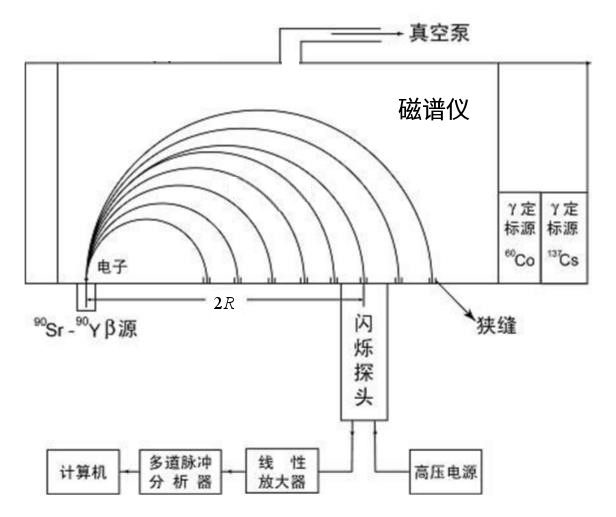
\includegraphics[height=12cm, width=14cm]{images/app.png}
 \caption{实验装置图}
 \label{fig:fig1}
\end{figure}\\\\
\end{itemize}

\newpage
\subsection{简要实验步骤}\label{sub:ExperimentalSteps}
分为以下几个步骤:\\\\
\circled{1}抽真空(按橘色按钮),约2分钟,机械泵声音平稳即可\\\\
\circled{2}将探测器的狭缝放最后一个窗,调节探测的高压(小于600V)或放大倍数,使得$\beta$的信号峰在屏幕的最右端完整显示出来\\\\
\circled{3}在真空状态下,将探测器放4或5号窗,加不同厚度的铝吸收片,测量并记录能谱(最后转为文本文件以便分析)及活时间,以便计算信号的计数率,给出计数率随铝片厚度(含无铝片)的变化,拟合出衰减常数\\\\
\circled{4}在等待的过程中,进行蒙特卡洛的模拟(注意根据实际实验装置更新磁场的磁感应强度及探测器所在窗的位置—输入狭缝中心所对的刻度尺读数)\\\\
\circled{5}在真空状态下,将探测器放2-8号窗,分别测量能谱,记下活时间及能谱(最后转为文本文件以便分析),以便计算信号的计数率。等待的过程中进行蒙特卡洛模拟。\\\\
\circled{6}关掉真空泵按钮。在等待真空盒进入空气的过程中,利用$\gamma$源进行探测器刻度。\\\\
\circled{7}等真空表指示为0的时候,在真空盒充满空气状态下重复步骤5。等待的过程中进行蒙特卡洛模拟。比较同一位置空气及真空下的计数率,计算出各能量下空气对$\beta$的衰减长度\\\\
\circled{8}将实验测量的$\beta$在空气与铝片中的衰减系数与蒙特卡洛模拟结果进行比较。\\\\



%%%%%%%%%%%%%%%%%%%%%%%%%%%%%%%%%%%%%%%% Results & Discussions %%%%%%%%%%%%%%%%%%%%%%%%%%%%%%%%%%%%%%%%
\newpage
\section{结果及讨论}

%------------------------------------------------------------
\subsection{真空状态下,信号计数率随铝片厚度的变化,拟合出衰减常数}\label{sub:alu}
加不同厚度的铝吸收片, 活时间$t=10min$,测量并记录能谱, 对不同厚度铝片测得能谱的本底用指数衰减函数拟合, 适当选择本底拟合区域, 然后在原始能谱中扣除本底得到信号分布, 如下图\ref{fig:fig2}. 
\begin{figure}[ht]
 \centering
 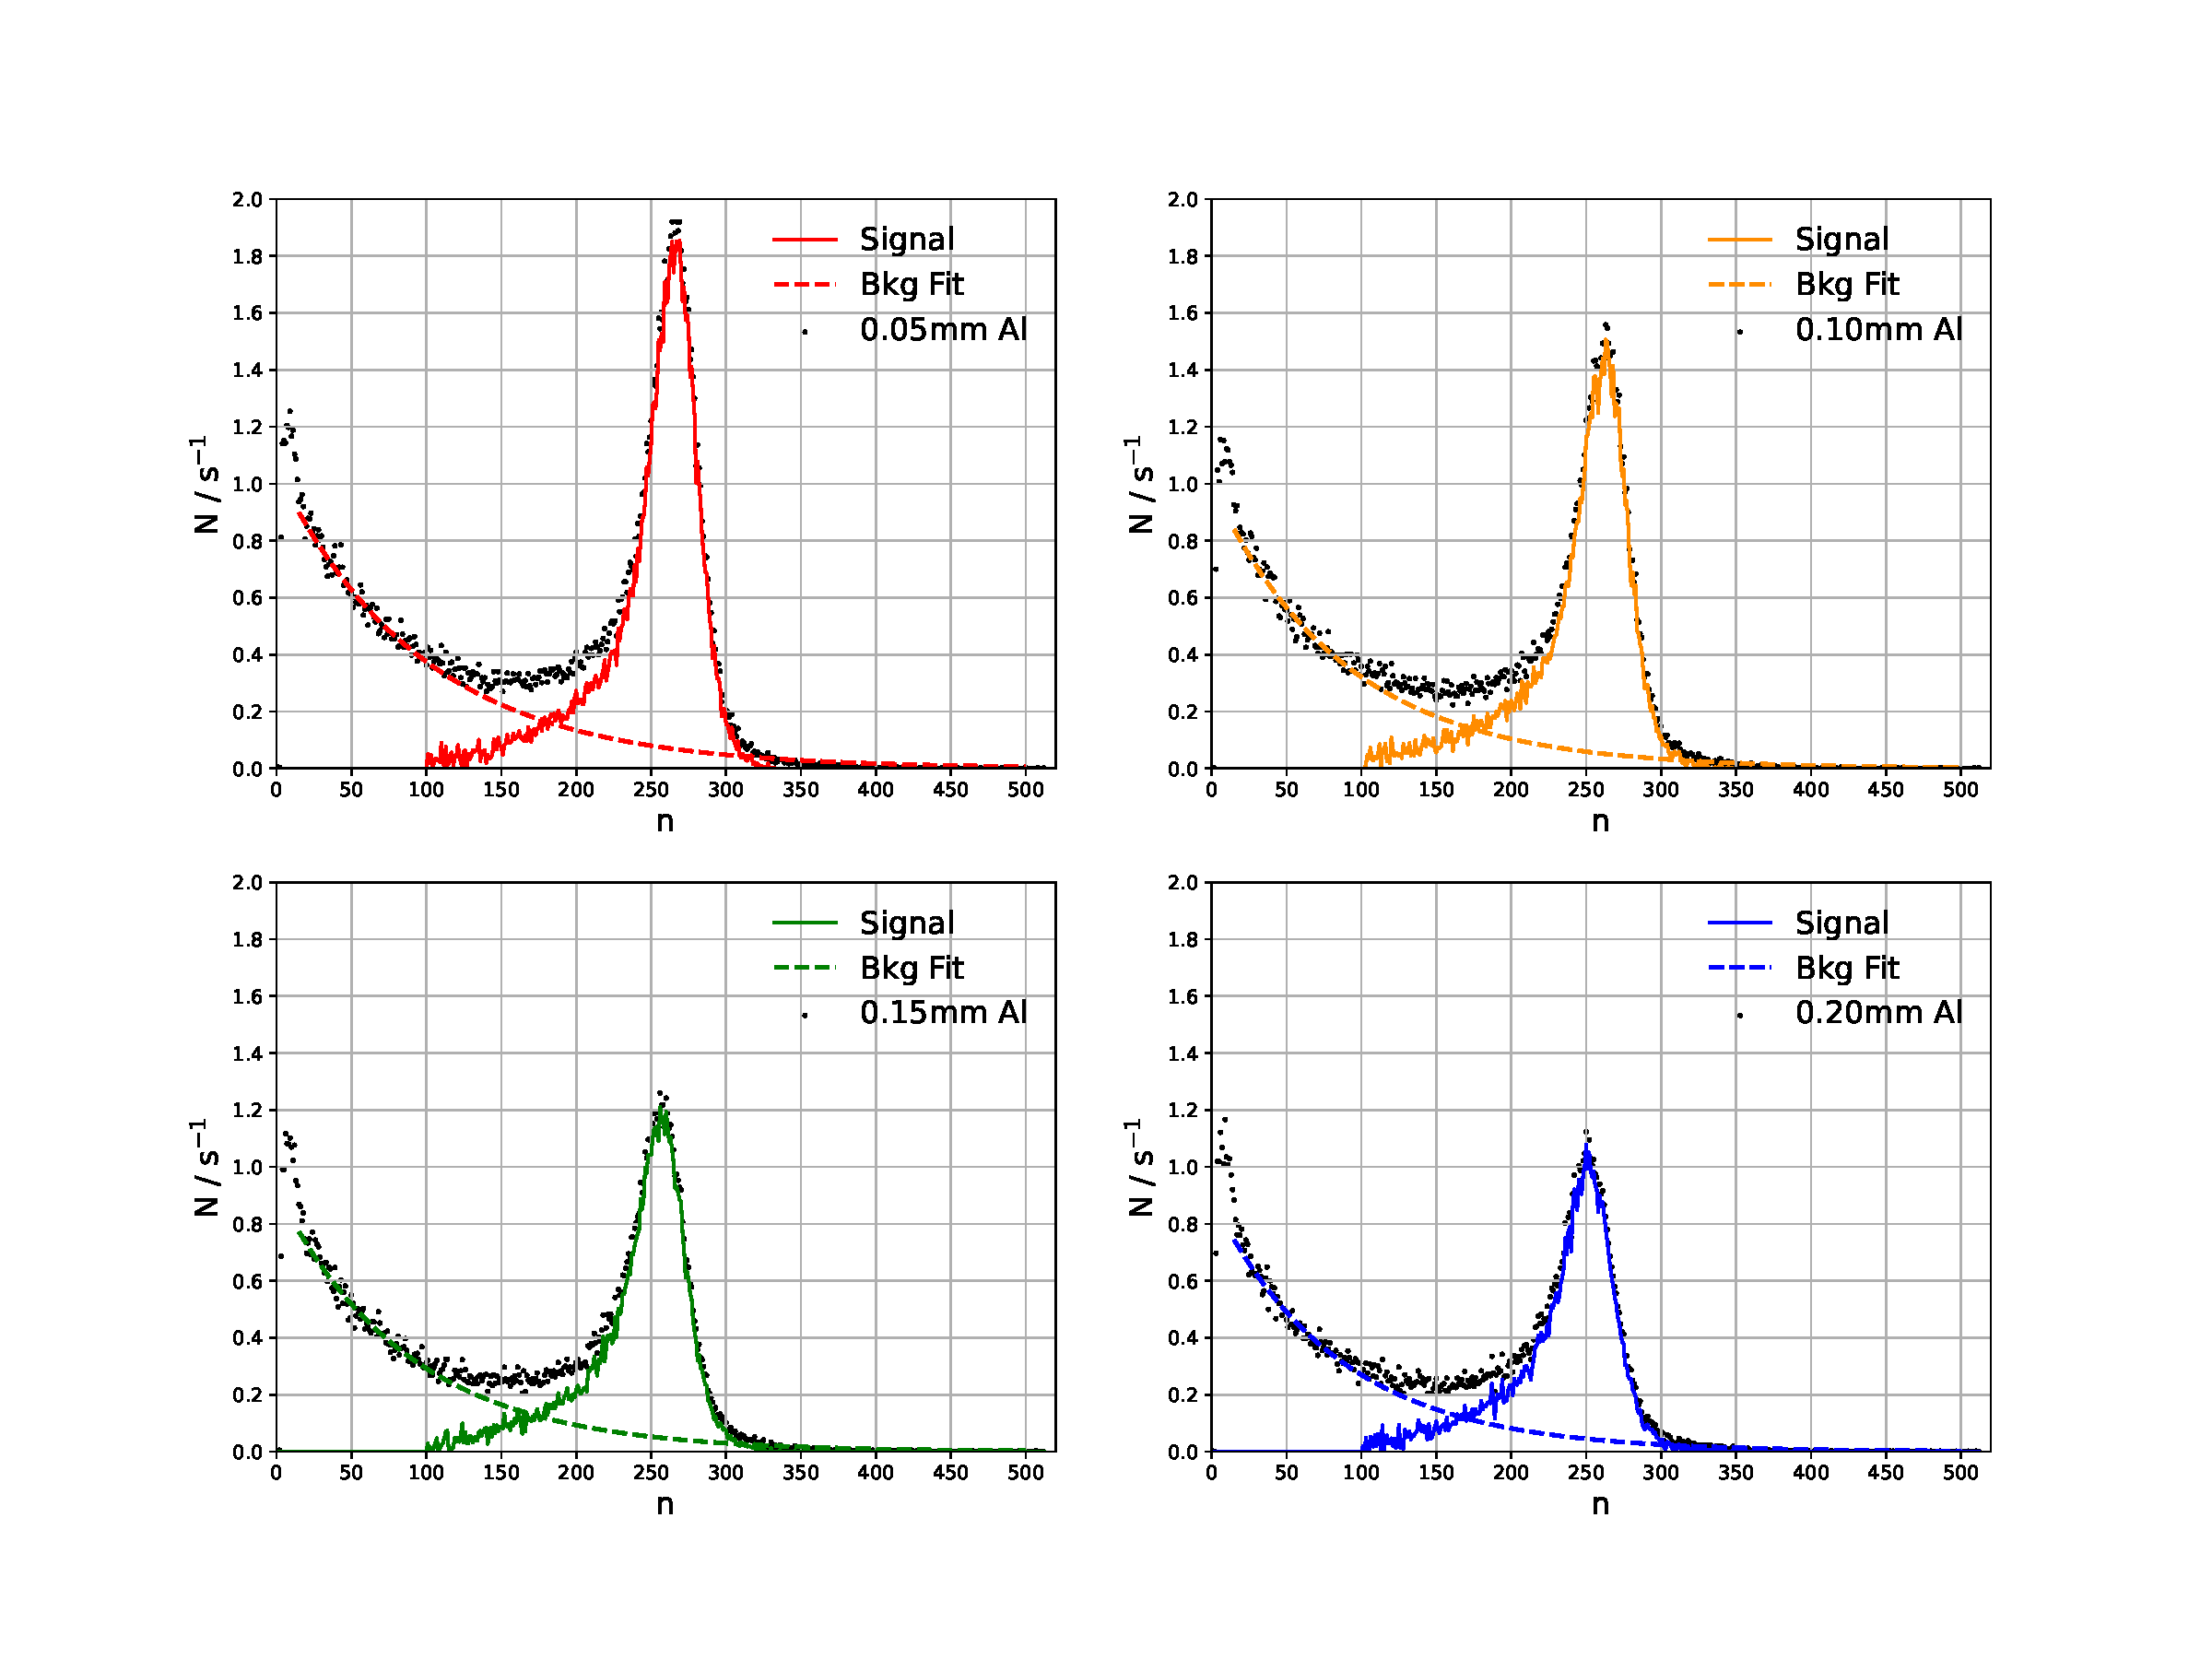
\includegraphics[height=12cm, width=16cm]{images/phyex1_fig3.pdf}
 \caption{原始能谱及拟合本底与信号分布}
 \label{fig:fig2}
\end{figure}\\\\
\newpage
信号计数率随铝片厚度的变化如下图\ref{fig:fig3}. 
\begin{figure}[ht]
 \centering
 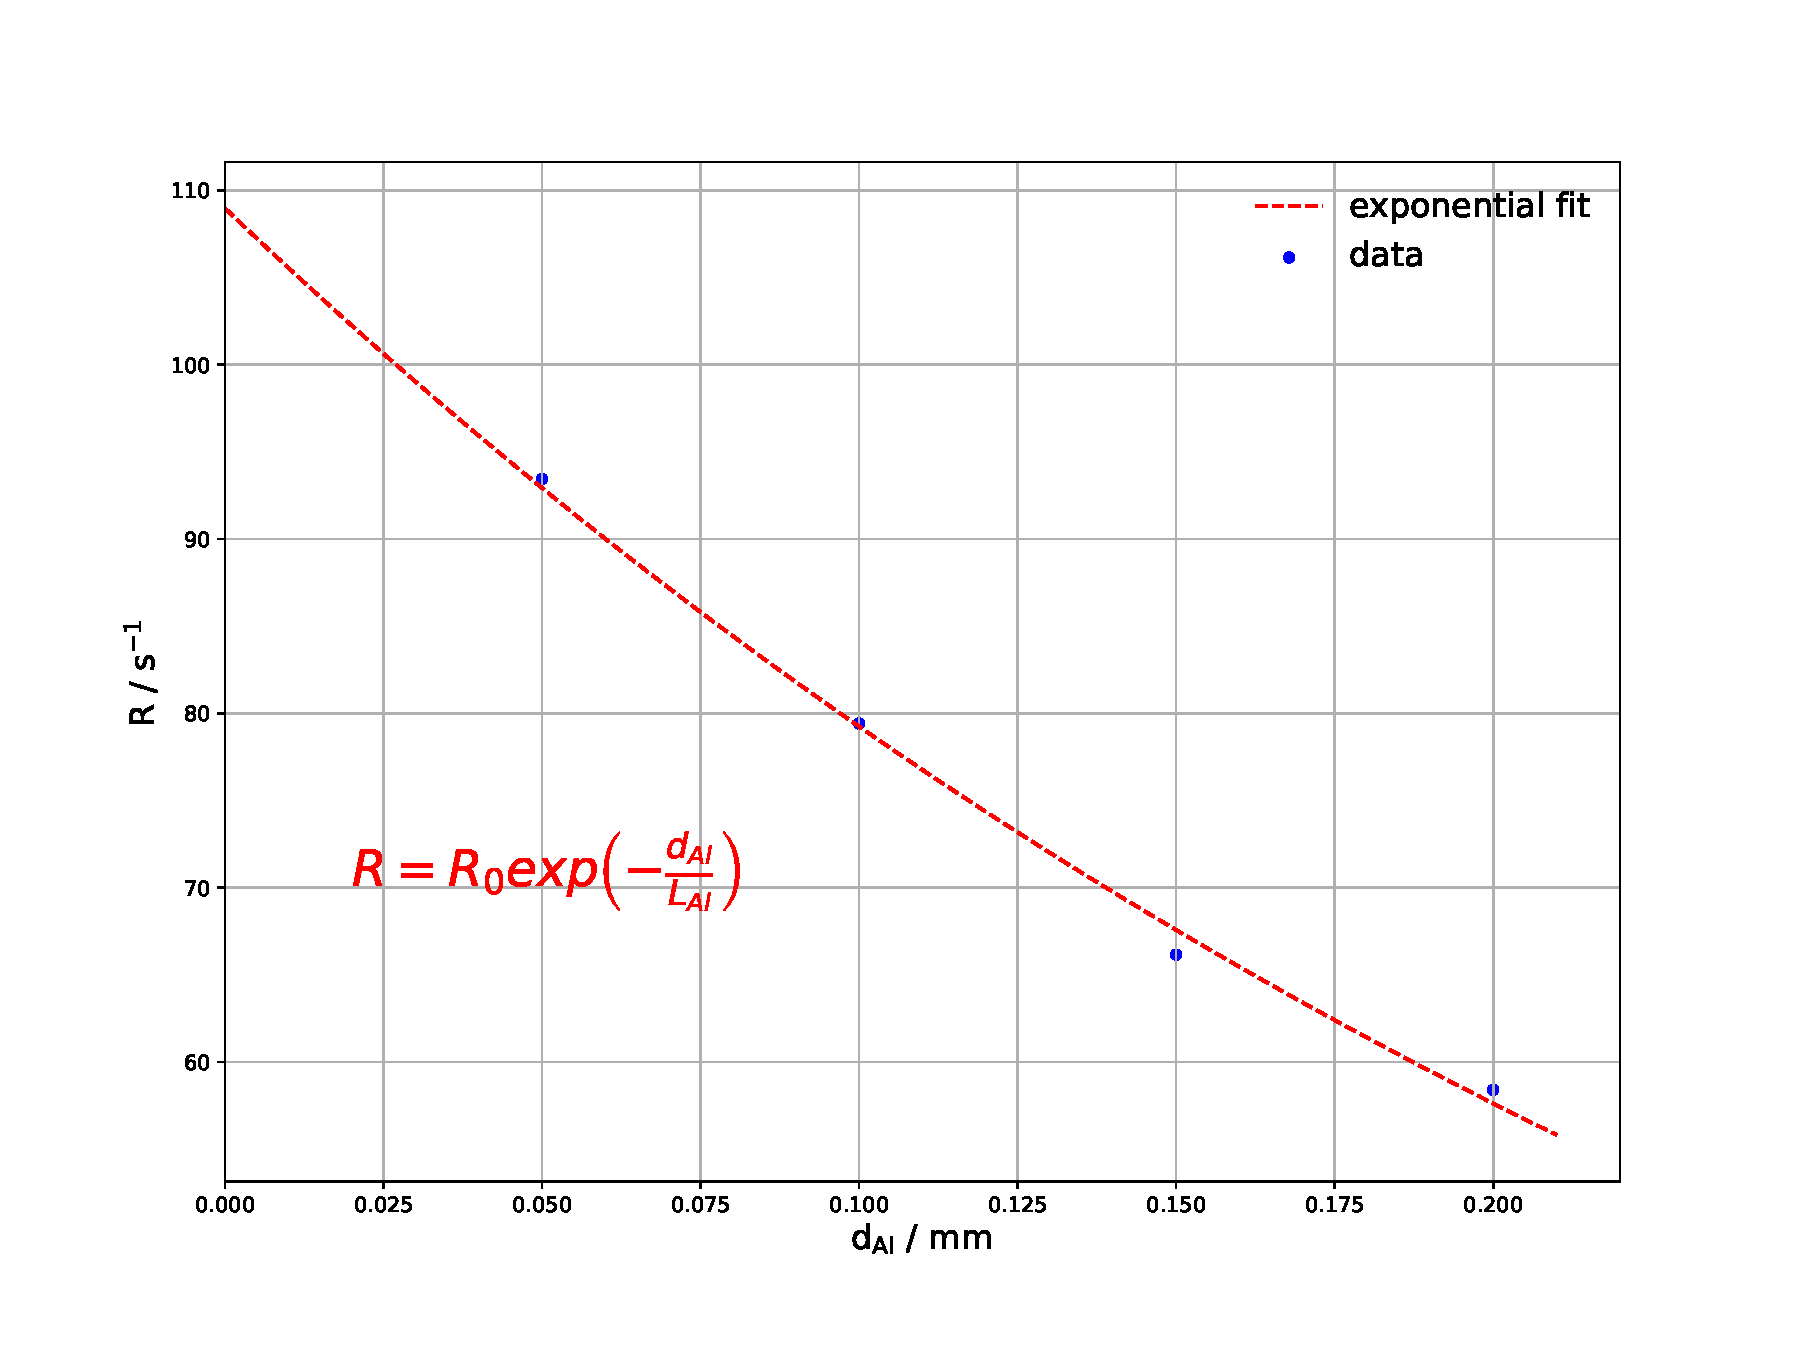
\includegraphics[height=12cm, width=16cm]{images/phyex1_fig4.pdf}
 \caption{信号计数率随铝片厚度的变化}
 \label{fig:fig3}
\end{figure}\\
通过拟合得到的结果和统计误差给出$\beta$射线在铝片中的衰减长度为
\begin{equation}
    L_{Al}\pm\sigma_{L_{Al}}=(0.31\pm0.02)mm
\end{equation}

\begin{comment}
如果需要索引参考文献,请使用\cite{Erdos01}, 同时已经将参考文献的项目模版在文末写出。
\end{comment}

%------------------------------------------------------------
\newpage
\subsection{利用$\gamma$源进行探测器刻度}\label{sub:ctl}
测出Co60与Cs137放射源的能谱图,并找到对应的光电峰, 如下图\ref{fig:fig4}. 
\begin{figure}[ht]
 \centering
 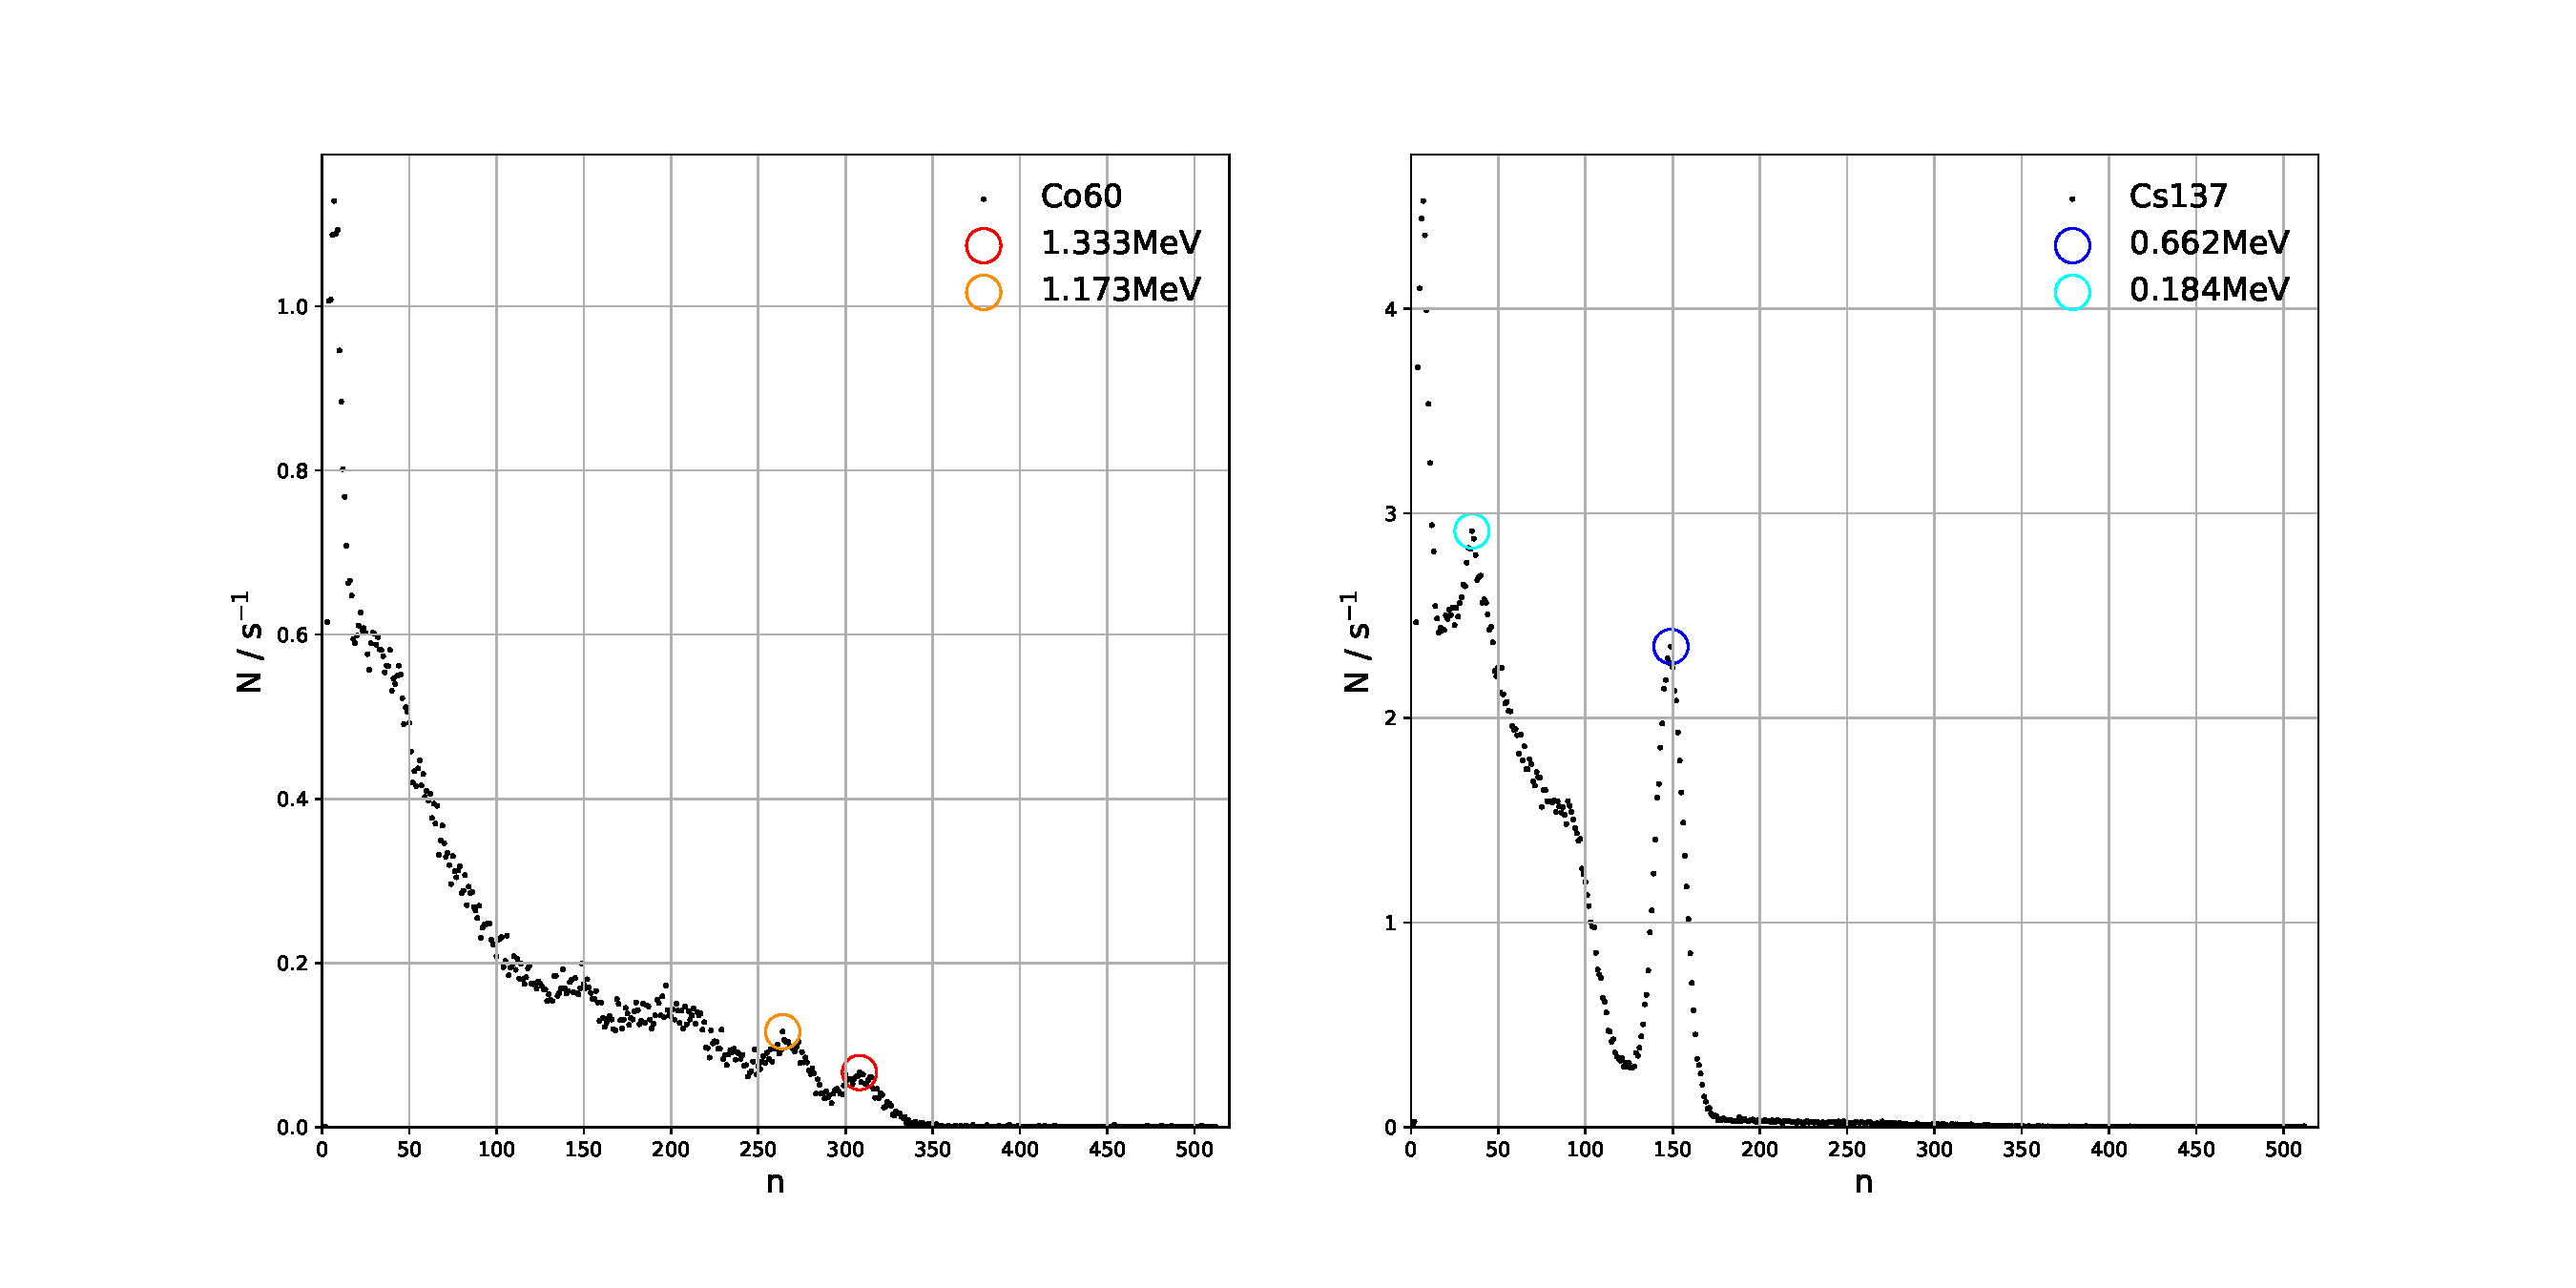
\includegraphics[height=8cm, width=16cm]{images/phyex3_fig1.pdf}
 \caption{Co60与Cs137的光电峰}
 \label{fig:fig4}
\end{figure}\\\\
可以得到入射光子的动能$E_k$与道数n的对应关系如下表
\begin{table}[htp]
\caption{道数n与动能$E_k$定量关系}\label{tab:signaldef}
\begin{center}\begin{tabular}{|l|l|l|p{6cm}|}
	\hline
	\textbf{道数$\rm n$} & \textbf{入射光子子动能$\rm E_k/MeV$}\\ \hline \hline
	$35$    & $0.184$ 	\\ \hline
	$149$    & $0.662$    \\ \hline
	$264$    & $1.173$    \\ \hline
	$308$    & $1.333$    \\ \hline
	\hline
	\end{tabular}
\end{center}
\end{table}\\
\newpage
利用线性拟合得到如下图刻度关系\ref{fig:fig5}. 
\begin{figure}[ht]
 \centering
 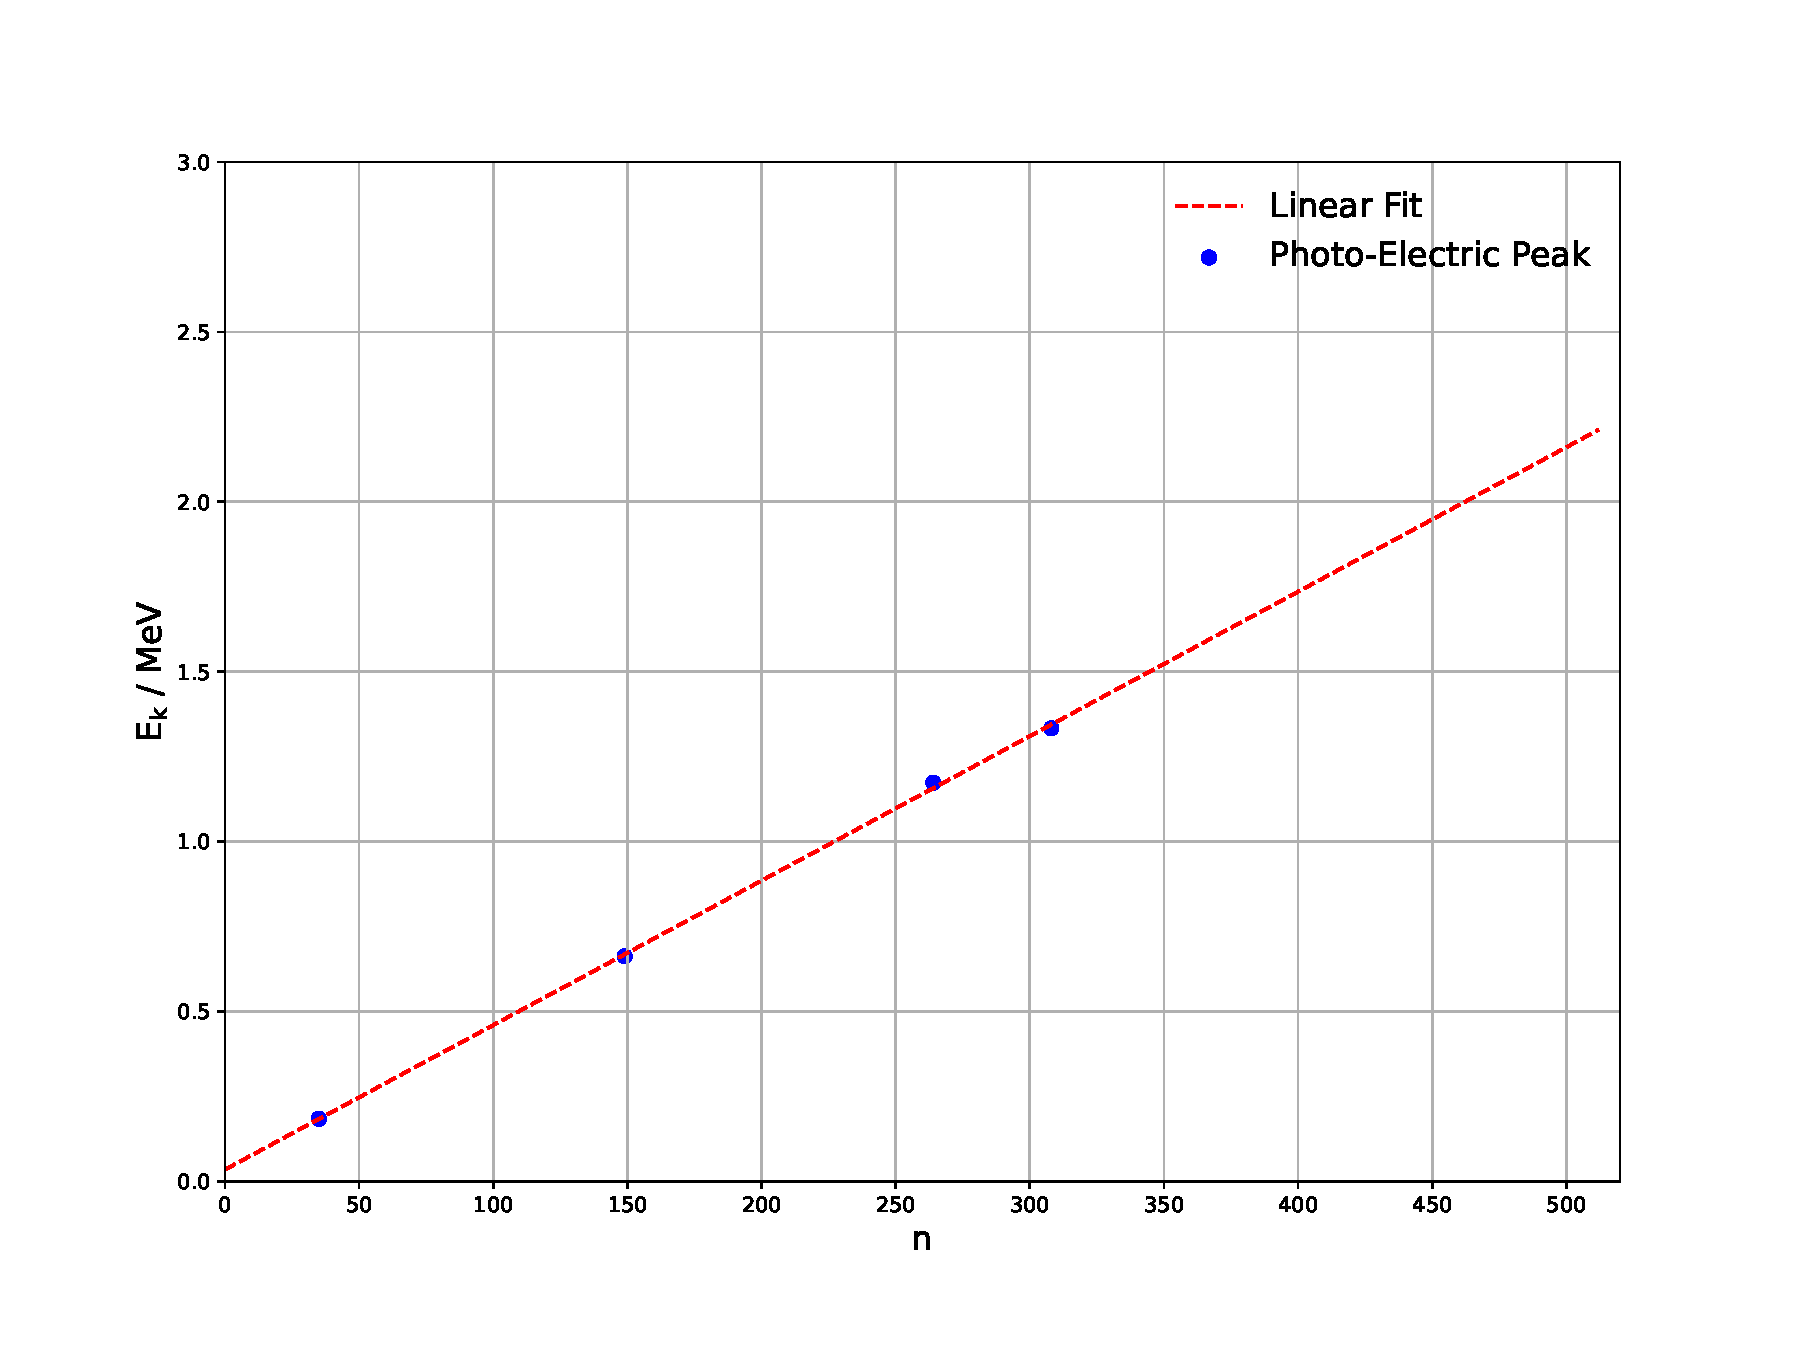
\includegraphics[height=12cm, width=16cm]{images/phyex3_fig2.pdf}
 \caption{利用$\gamma$源对探测器刻度}
 \label{fig:fig5}
\end{figure}\\
通过最小二乘法, 我们可以得到刻度的线性关系以及参数的统计误差如下
\begin{equation}
    E_k=kn+b
\end{equation}
此处
\begin{equation}
k=(0.00425\pm0.00007)\rm MeV
\end{equation}
\begin{equation}
b=(0.03432\pm0.01472)\rm MeV
\end{equation}

%------------------------------------------------------------
\newpage
\subsection{计算各能量下空气对$\beta$粒子的衰减长度}
将探测器放2-8号窗,活时间$t=10min$我们分别在真空状态下与空气状态下测量能谱,与探测器位置的关系如下图\ref{fig:fig5}所示. 
\begin{figure}[ht]
 \centering
 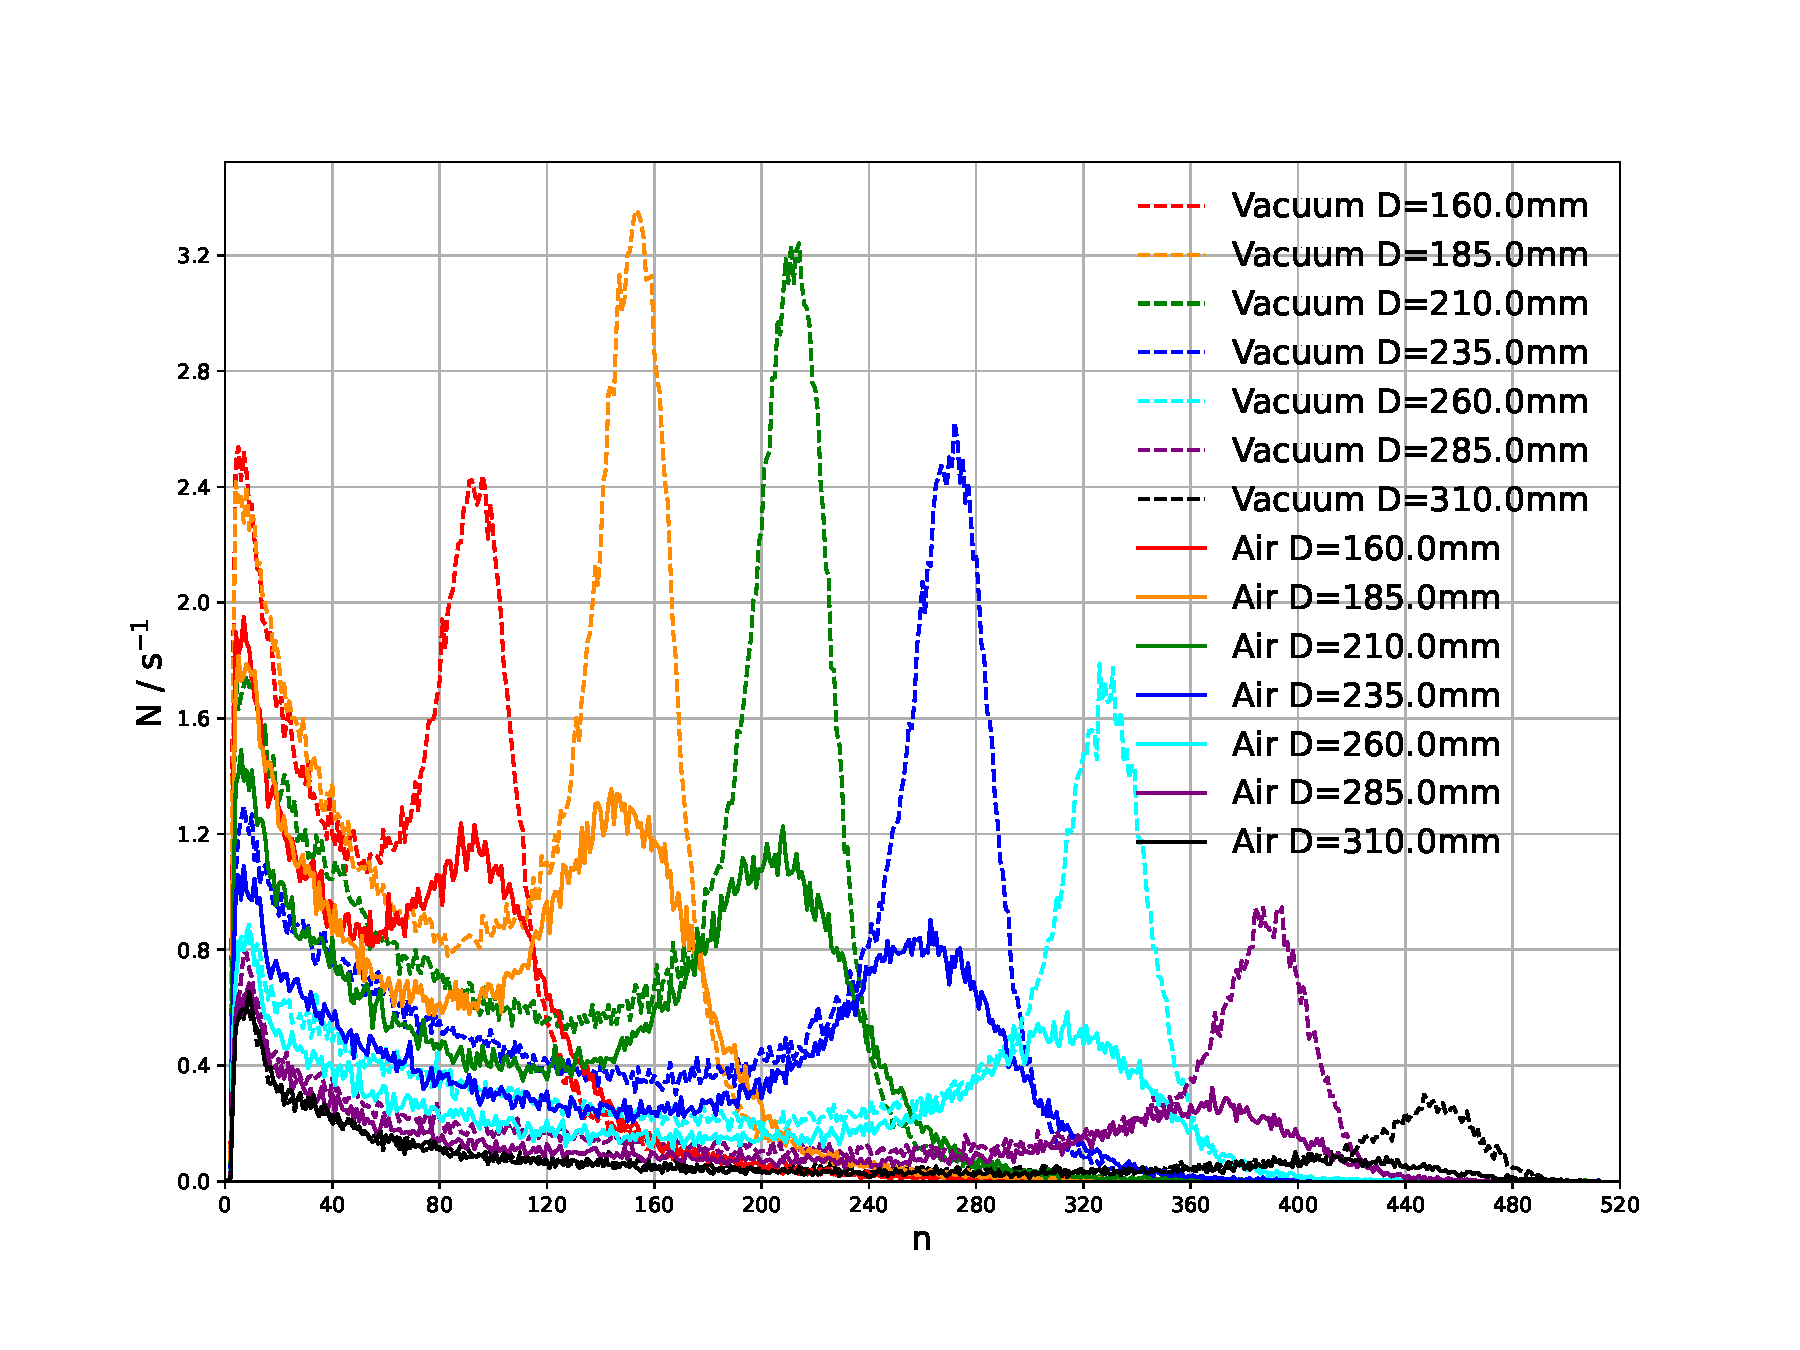
\includegraphics[height=12cm, width=16cm]{images/phyex5_fig1.pdf}
 \caption{原始能谱和信号分布随探测器位置变化}
 \label{fig:fig5}
\end{figure}\\
利用同前面类似的方法指数衰减来拟合本底, 用原始能谱扣除本底即可得到信号分布和信号计数率
\newpage
利用
\begin{equation}
L_A=\frac{x}{\ln{\frac{R_V}{R_A}}}
\end{equation}

以及
\begin{equation}
    p=eBR=\frac{1}{2}eBD
\end{equation}
\begin{equation}
    E_k=\sqrt{p^2c^2+m^2c^4}-mc^2    
\end{equation}


可以算出空气对$\beta$粒子的衰变长度$L_A$与其动能$E_k$的关系如图\ref{fig:fig6}. 
\begin{figure}[ht]
 \centering
 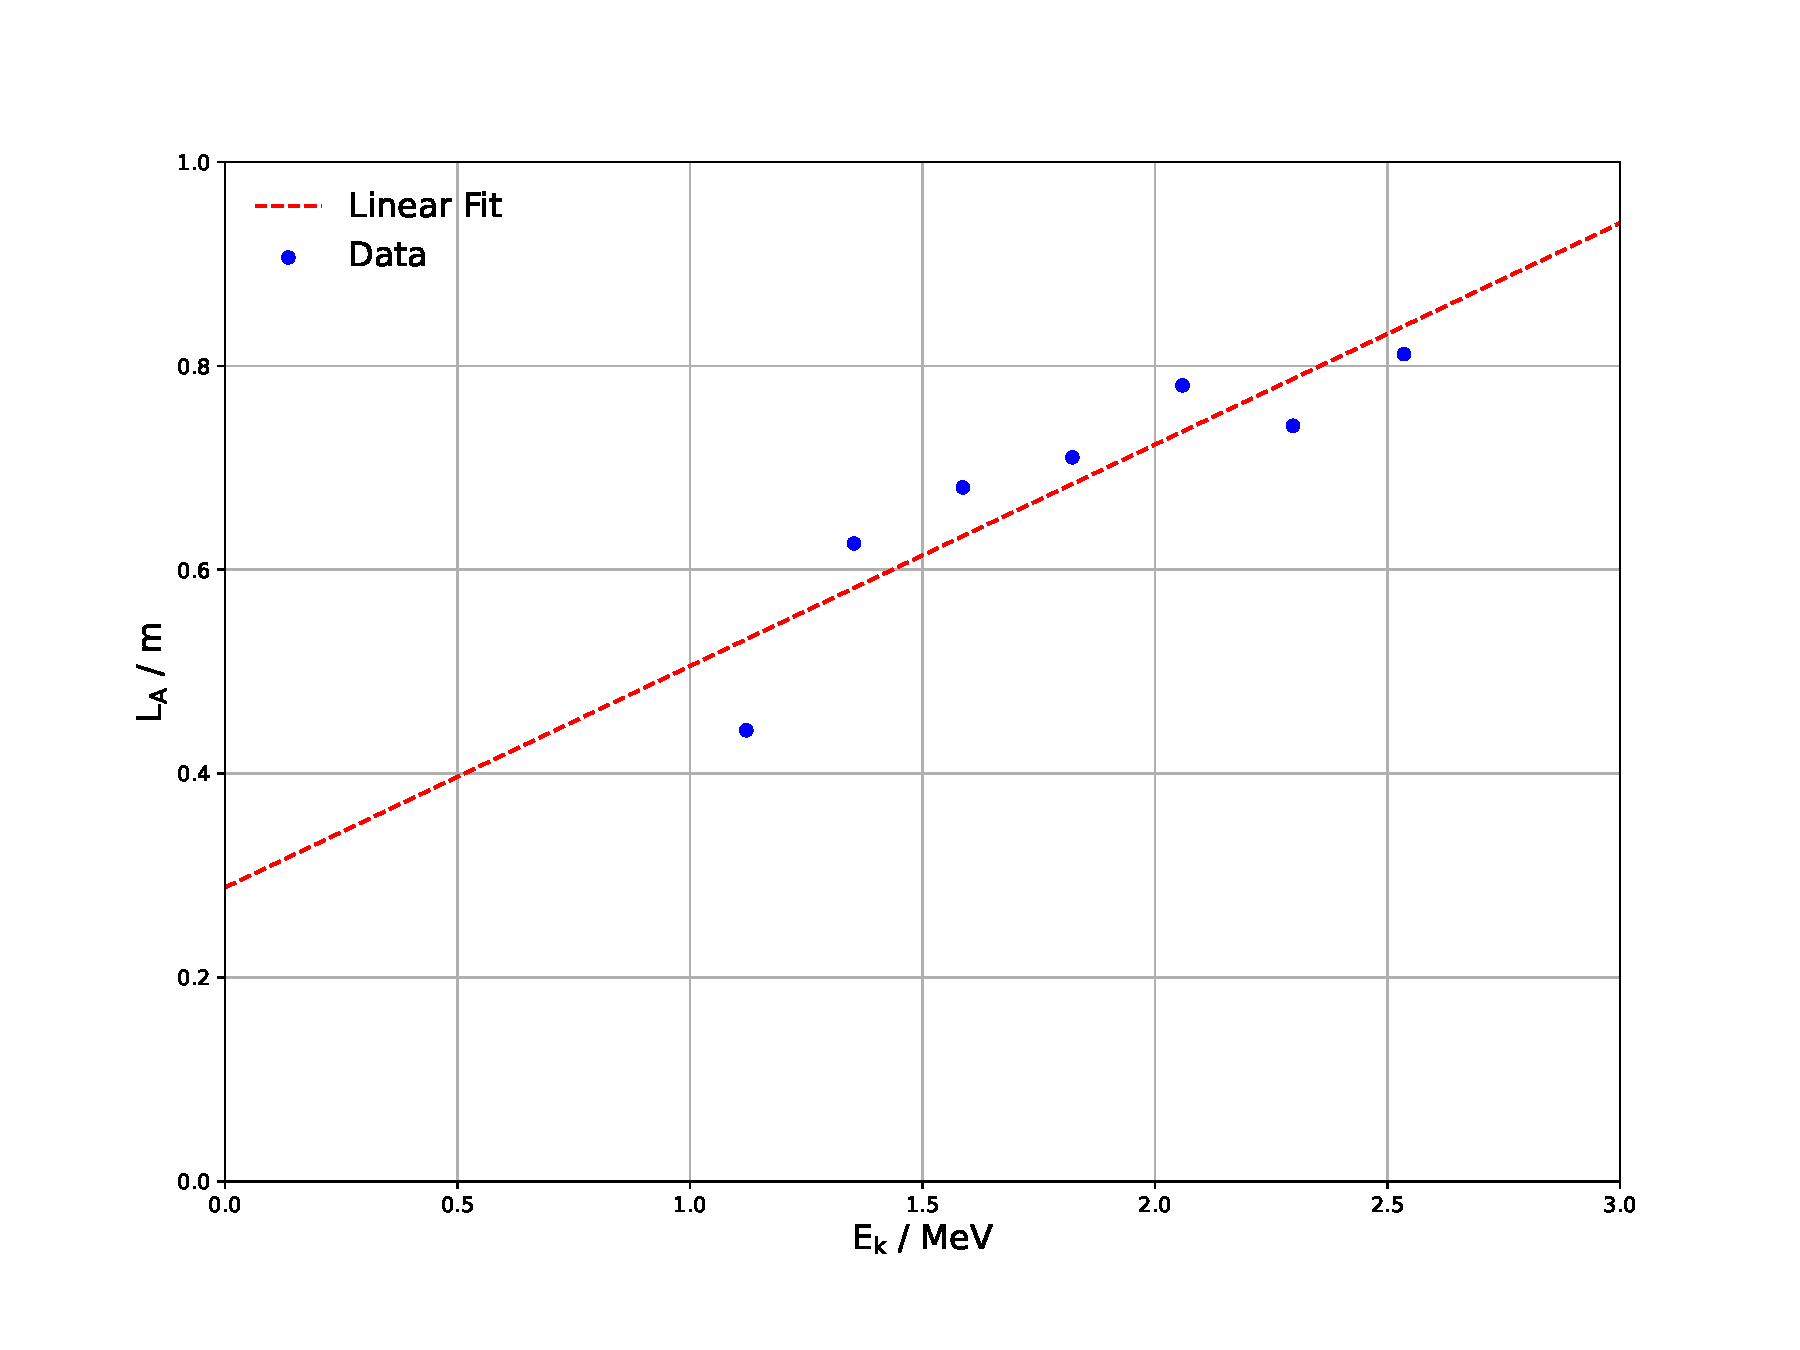
\includegraphics[height=12cm, width=16cm]{images/phyex5_fig3.pdf}
 \caption{空气对不同动能的$\beta$射线的衰减长度}
 \label{fig:fig6}
\end{figure}\\
可以看出能量越大, $\beta$射线的穿透能力越强, 即衰减长度的数值越大
\newpage
%------------------------------------------------------------
\subsection{用蒙特卡洛模拟重复上述实验过程}\label{sub:pulsewave}
\subsubsection{真空状态下,信号计数率随铝片厚度的变化,拟合出衰减常数}
利用蒙特卡洛方法模拟不同厚度铝片对$\beta$射线的衰减作用, 利用同前面类似的方法指数衰减来拟合本底, 得到原始能谱和信号分布如下图\ref{fig:fig7}. 
\begin{figure}[ht]
 \centering
 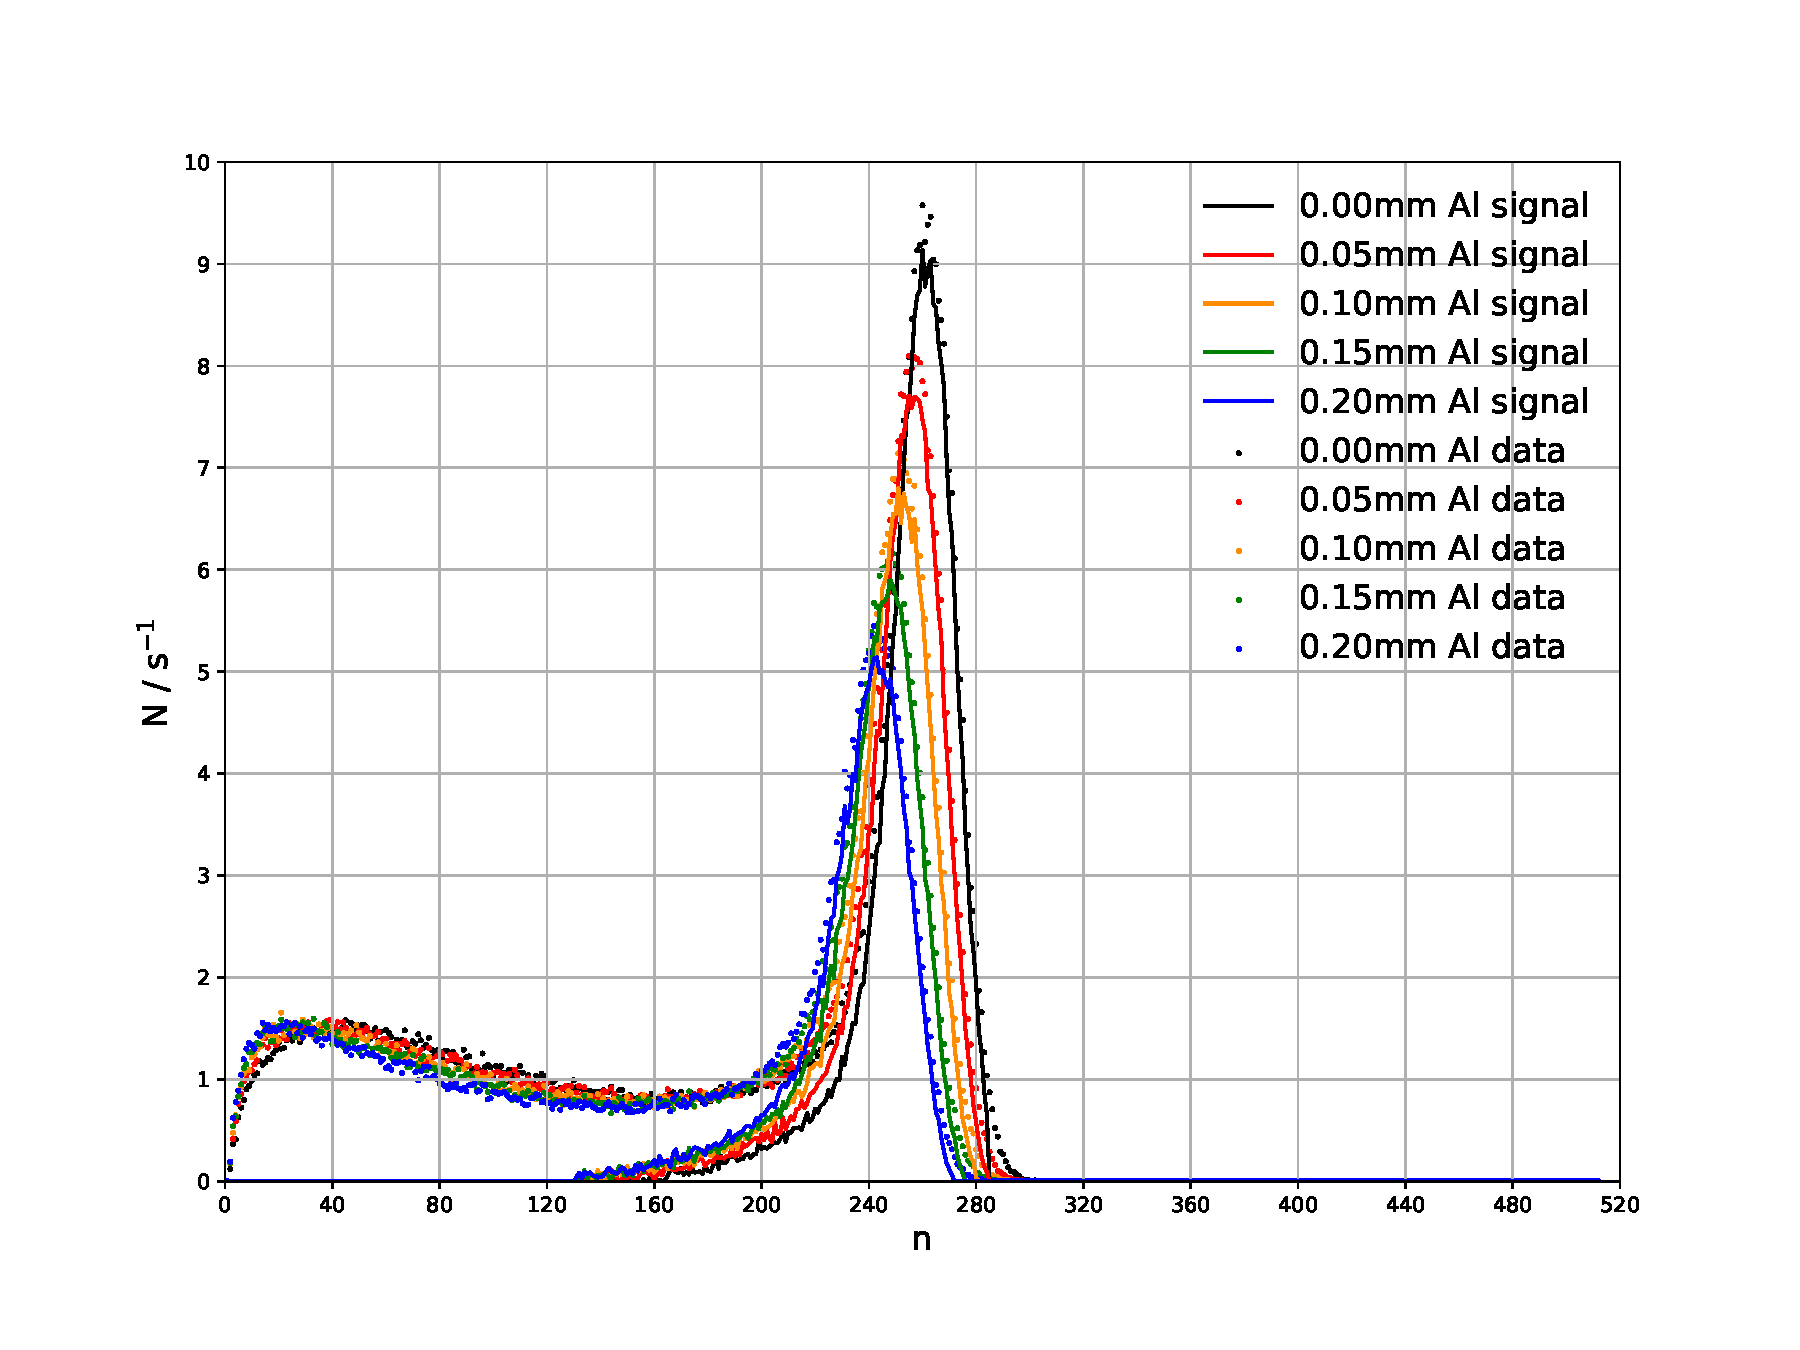
\includegraphics[height=12cm, width=16cm]{images/phyex2_fig1.pdf}
 \caption{蒙卡模拟的原始能谱与信号分布}
 \label{fig:fig7}
\end{figure}\\
\newpage
然后作出信号计数率随铝片厚度的变化关系图, 并用指数衰减拟合,如下图\ref{fig:fig8}. 
\begin{figure}[ht]
 \centering
 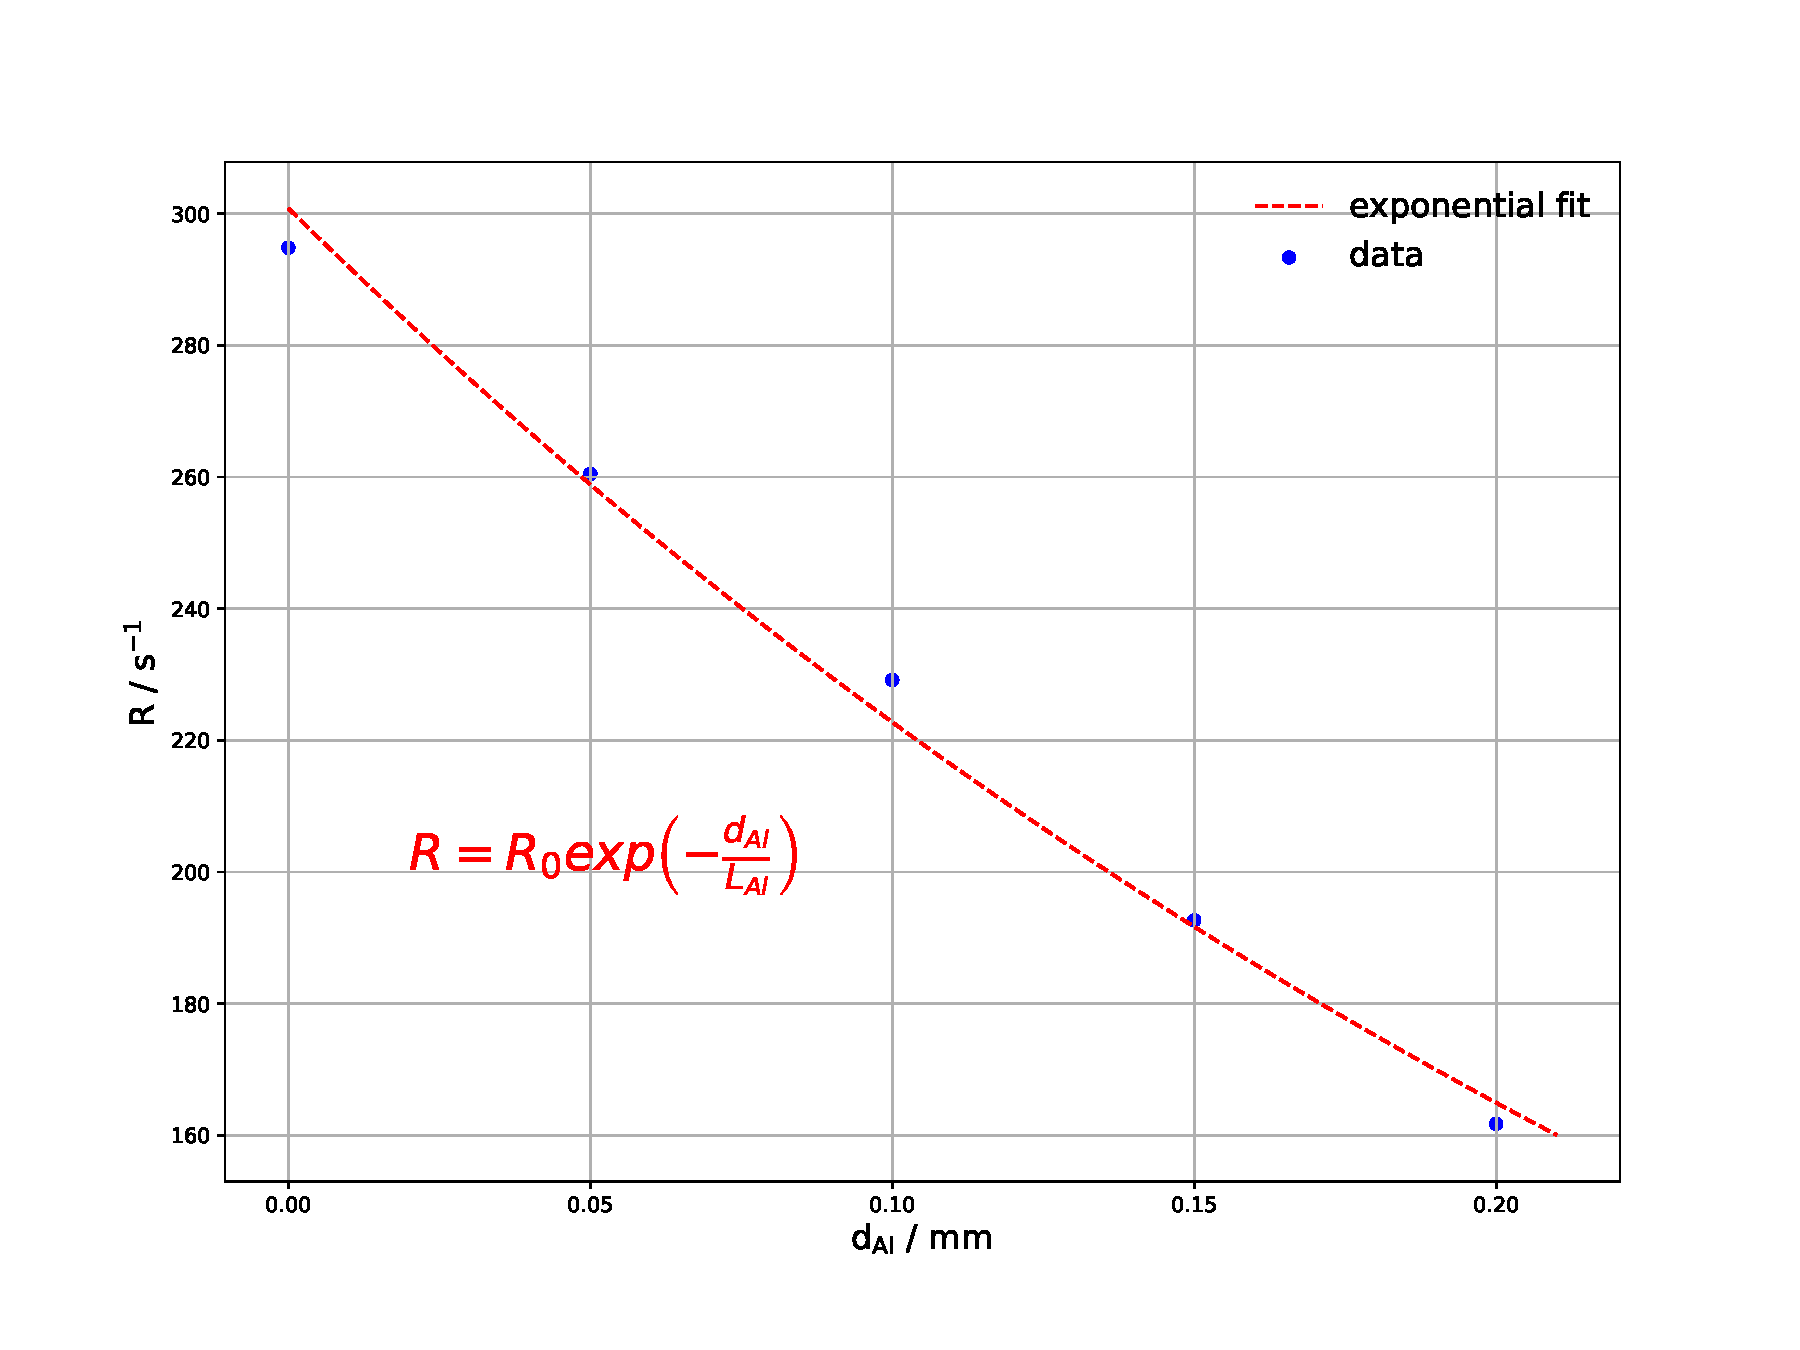
\includegraphics[height=12cm, width=16cm]{images/phyex2_fig2.pdf}
 \caption{蒙卡模拟的信号计数率随铝片厚度变化}
 \label{fig:fig8}
\end{figure}\\\\
通过拟合得到的结果和统计误差给出$\beta$射线在铝片中的衰减长度为
\begin{equation}
    L_{Al}\pm\sigma_{L_{Al}}=(0.33\pm0.02)mm
\end{equation}
蒙卡模拟的结果与前面用实验数据测出来的结果十分接近.
\newpage
\subsubsection{利用$\gamma$源进行探测器刻度}
蒙卡模拟出Co60与Cs137放射源的能谱图,并找到对应的光电峰, 如下图\ref{fig:fig9}. 
\begin{figure}[ht]
 \centering
 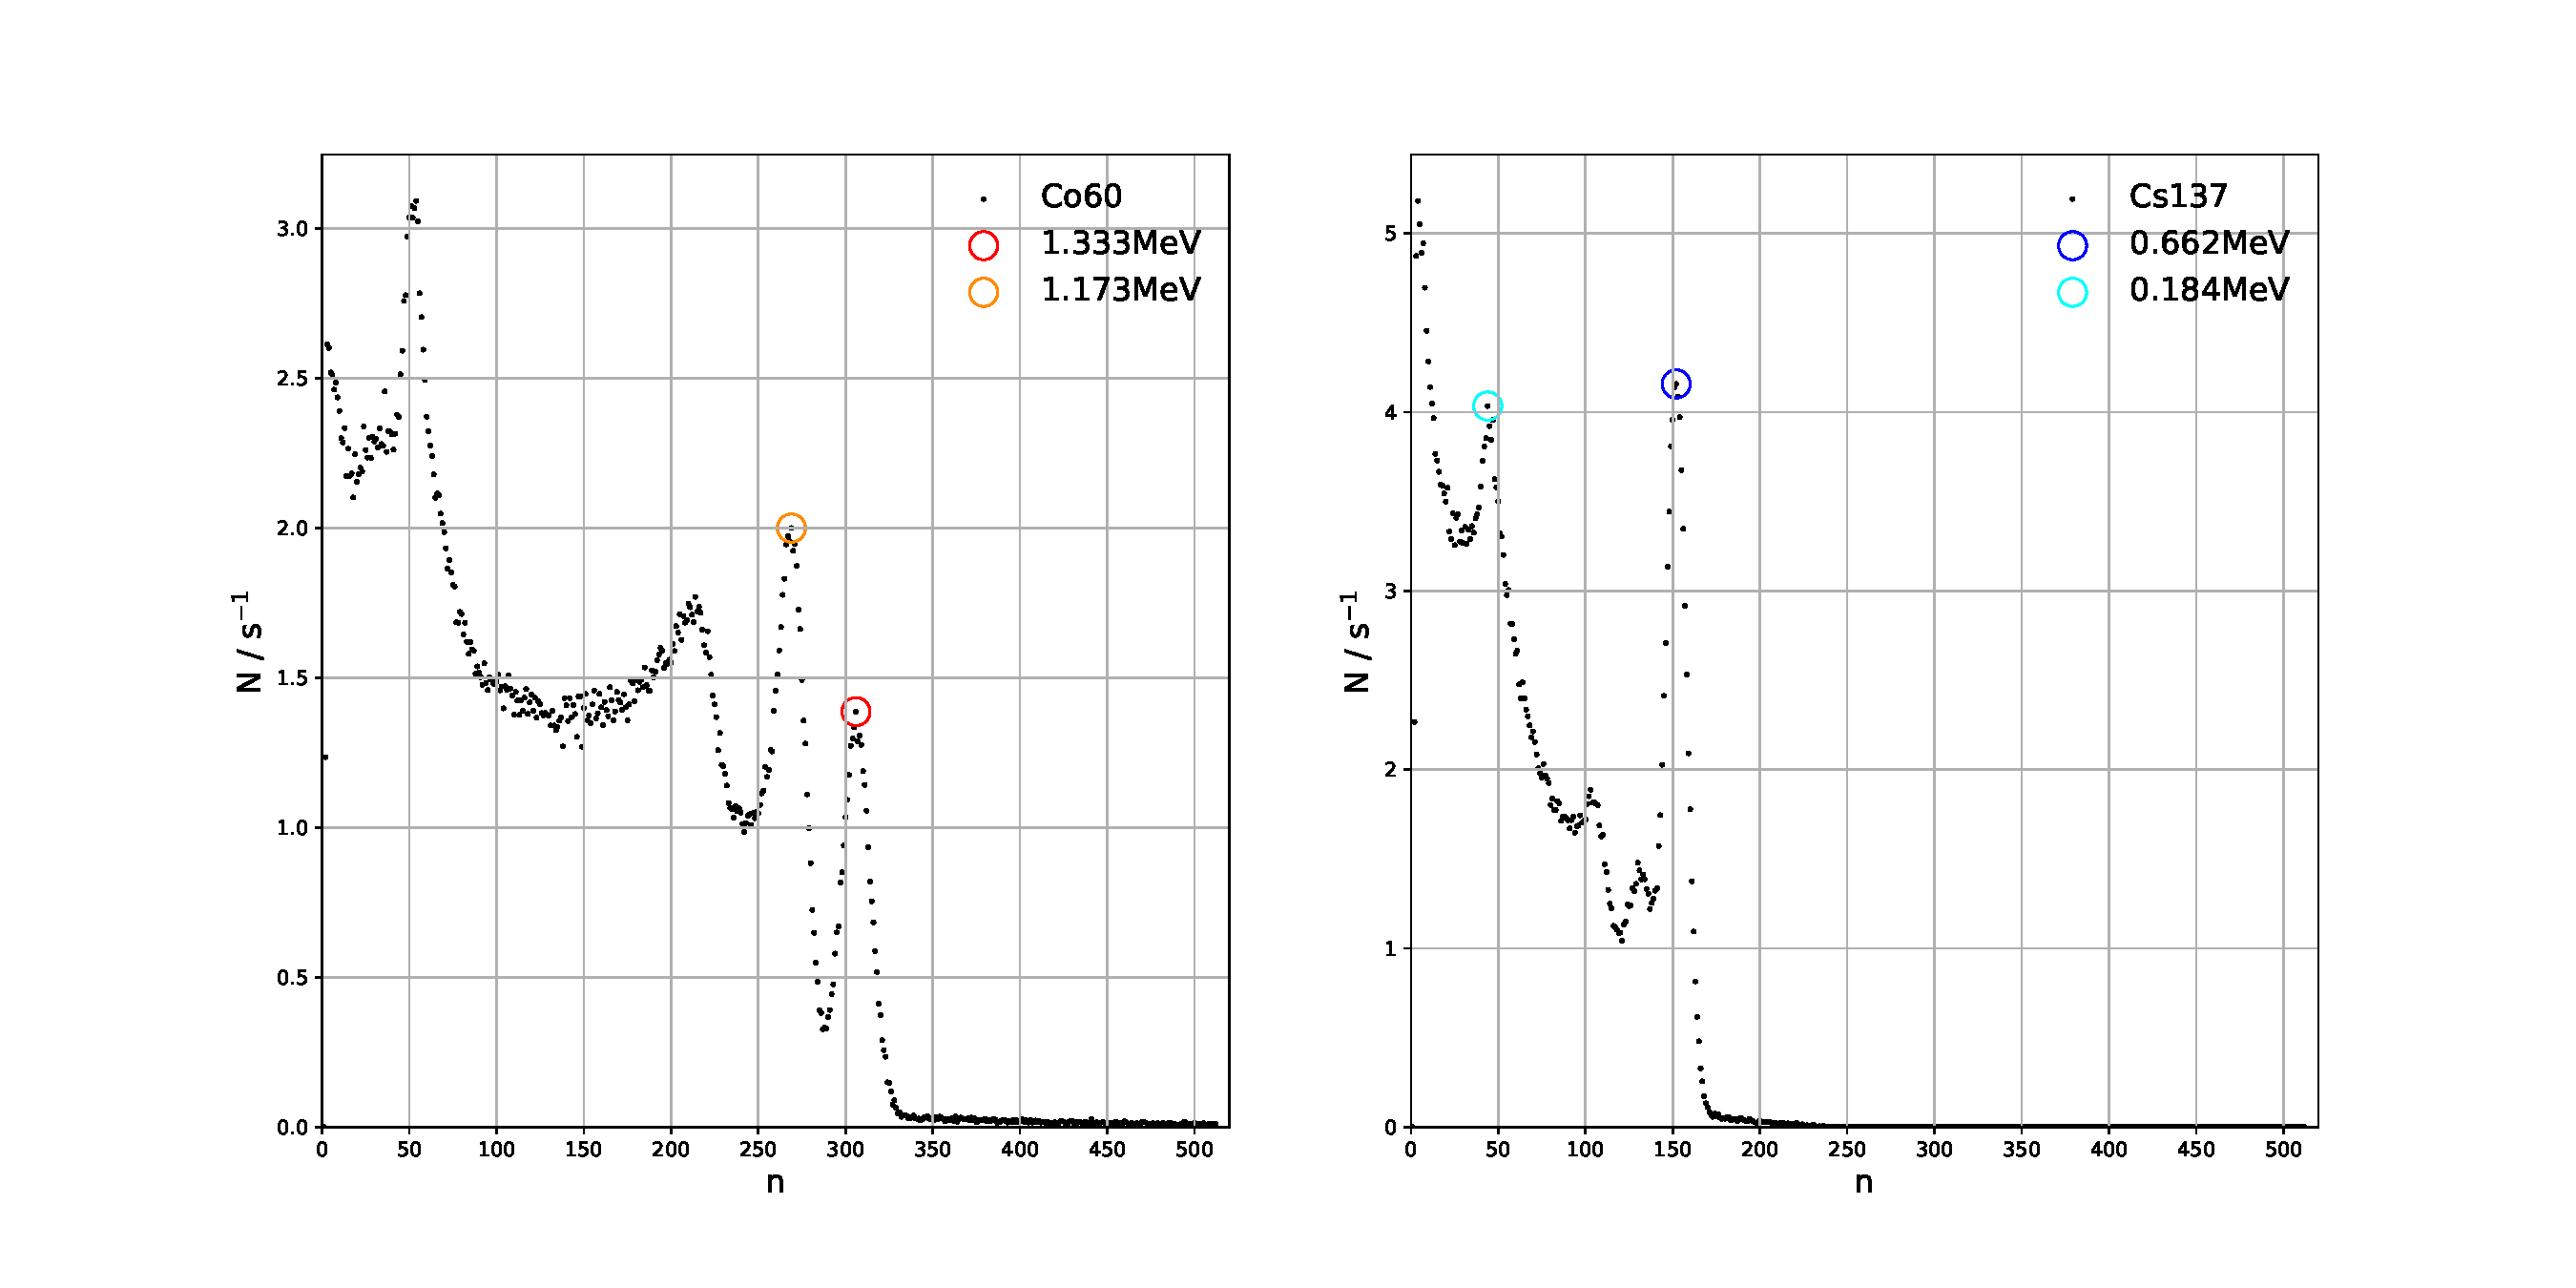
\includegraphics[height=8cm, width=16cm]{images/phyex4_fig1.pdf}
 \caption{Co60与Cs137的光电峰}
 \label{fig:fig9}
\end{figure}\\\\
可以得到模拟的入射光子的动能$E_k$与道数n的对应关系如下表
\begin{table}[htp]
\caption{道数n与动能$E_k$定量关系}\label{tab:signaldef}
\begin{center}\begin{tabular}{|l|l|l|p{6cm}|}
	\hline
	\textbf{道数$\rm n$} & \textbf{入射光子子动能$\rm E_k/MeV$}\\ \hline \hline
	$44$    & $0.184$ 	\\ \hline
	$152$    & $0.662$    \\ \hline
	$269$    & $1.173$    \\ \hline
	$306$    & $1.333$    \\ \hline
	\hline
	\end{tabular}
\end{center}
\end{table}\\
\newpage
尝试通过蒙卡模拟的过程对探测器进行刻度, 如下图\ref{fig:fig10}. 
\begin{figure}[ht]
 \centering
 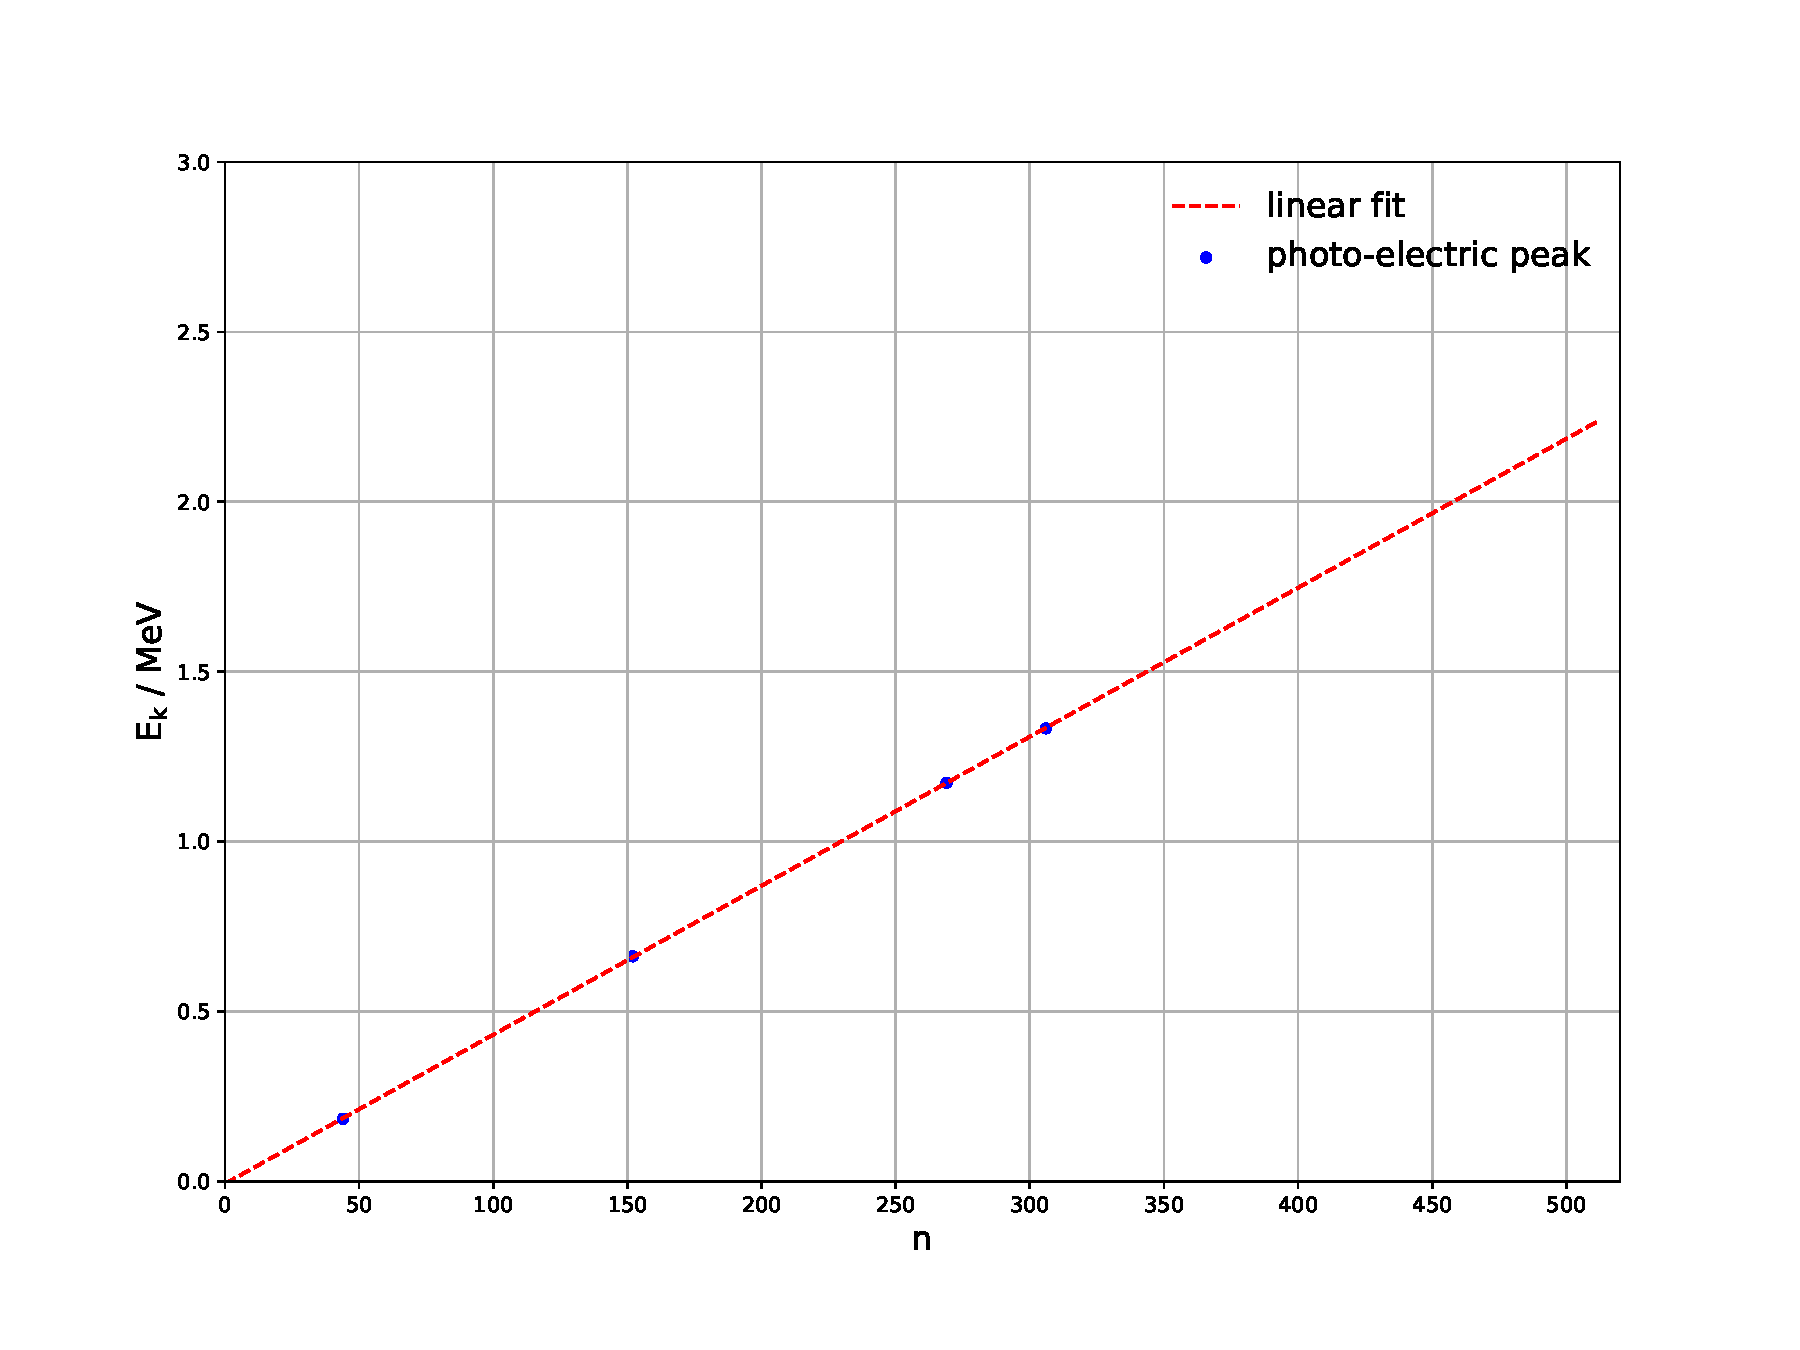
\includegraphics[height=12cm, width=16cm]{images/phyex4_fig2.pdf}
 \caption{利用$\gamma$源对探测器刻度}
 \label{fig:fig10}
\end{figure}\\
通过最小二乘法, 我们可以得到模拟出的刻度的线性关系以及参数的统计误差如下
\begin{equation}
    E_k=kn+b
\end{equation}
此处
\begin{equation}
k=(0.00439\pm0.00001)\rm MeV
\end{equation}
\begin{equation}
b=(-0.00728\pm0.00273)\rm MeV
\end{equation}
可以看到蒙卡模拟的结果与前面用实验数据测出来的结果十分接近.
\newpage

\subsubsection{计算各能量下空气对$\beta$粒子的衰减长度}
蒙卡模拟出的$\beta$射线在真空中与空气中的能谱分布如下图\ref{fig:fig11}. 
\begin{figure}[ht]
 \centering
 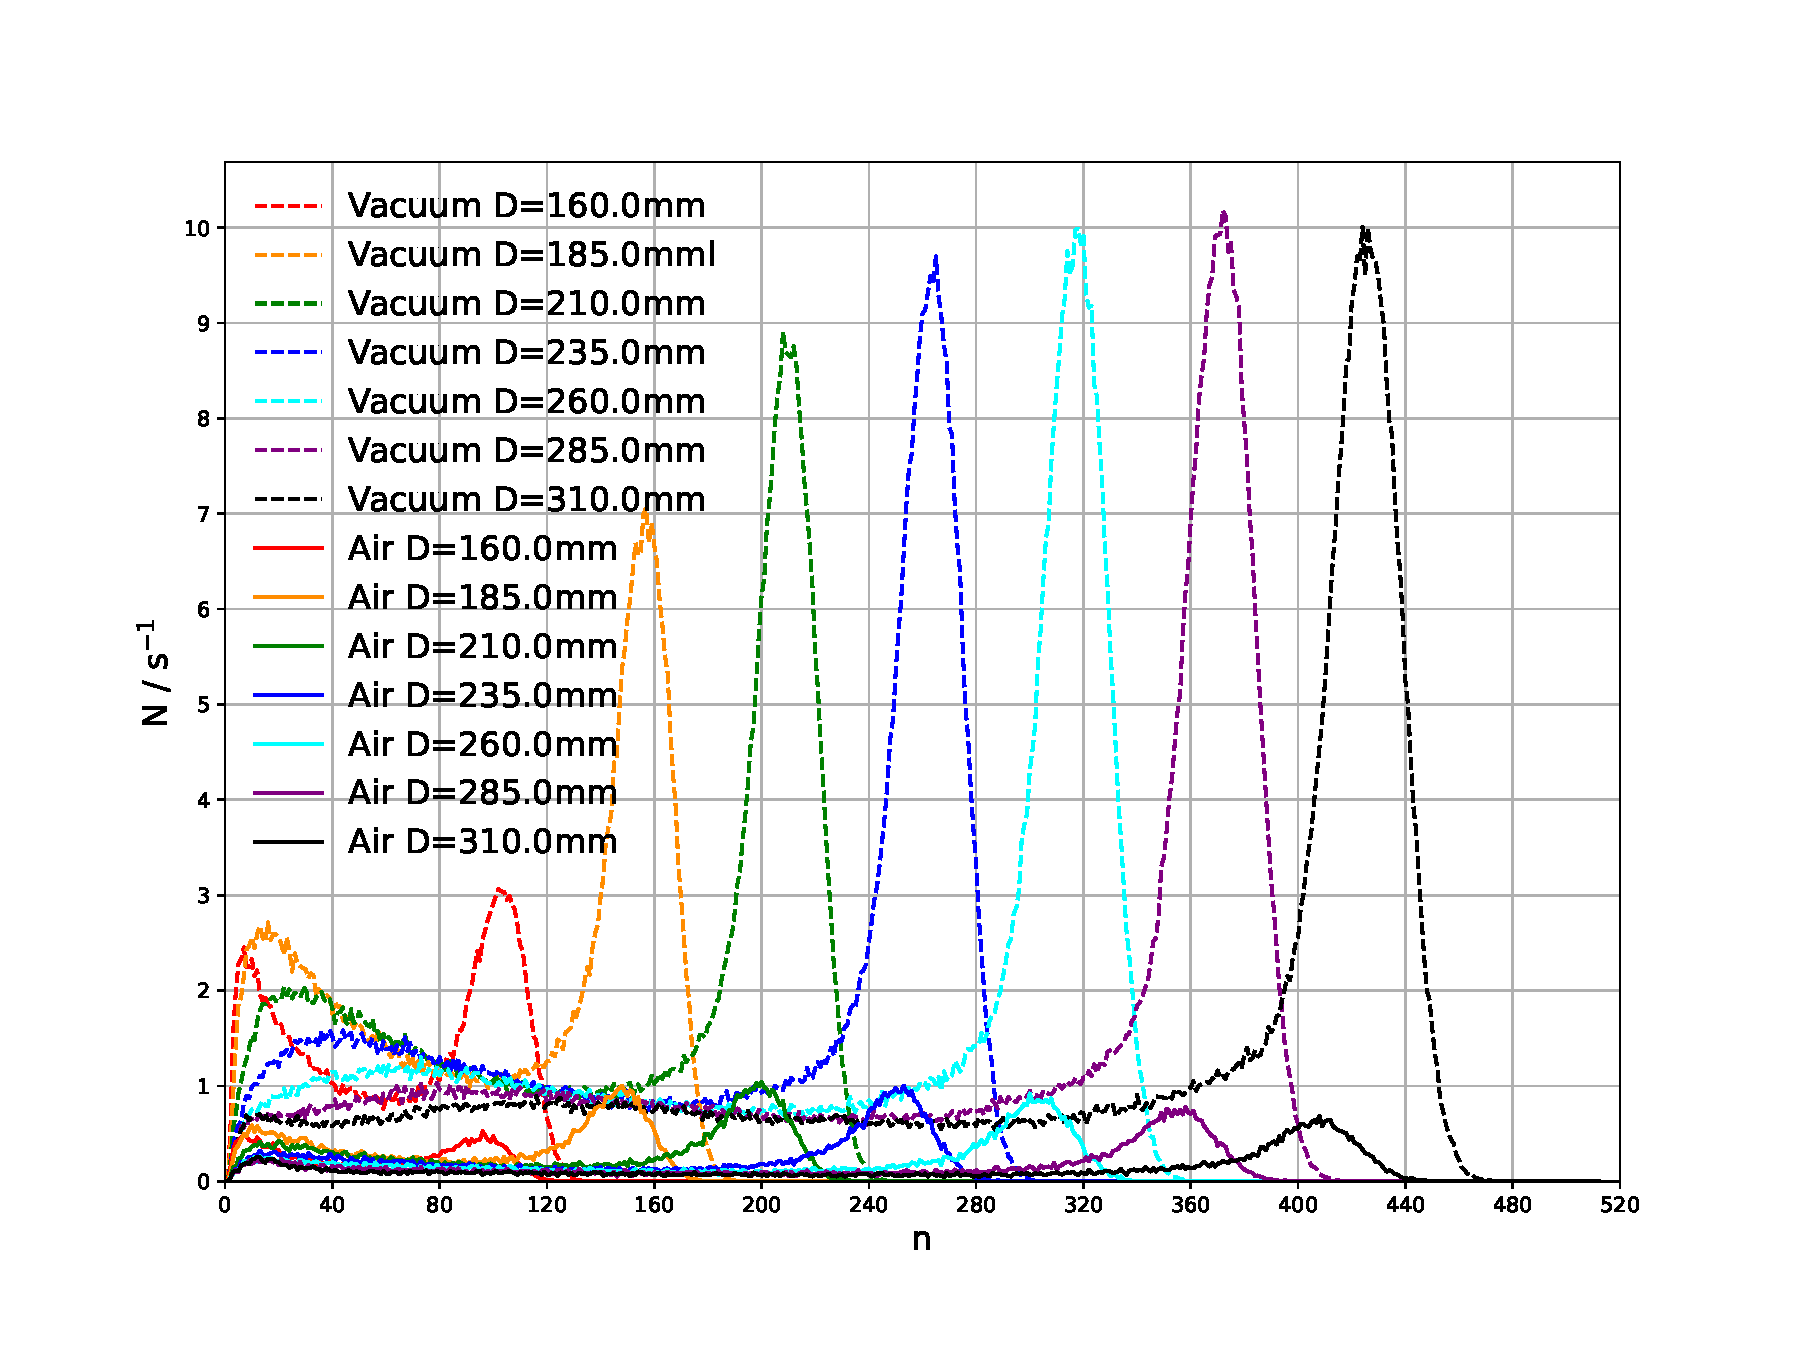
\includegraphics[height=12cm, width=16cm]{images/phyex6_fig1.pdf}
 \caption{蒙卡模拟真空与空气中$\beta$的能谱分布}
 \label{fig:fig11}
\end{figure}\\\\
\newpage

可以算出空气对$\beta$粒子的衰变长度$L_A$与其动能$E_k$的关系如图\ref{fig:fig12}. 
\begin{figure}[ht]
 \centering
 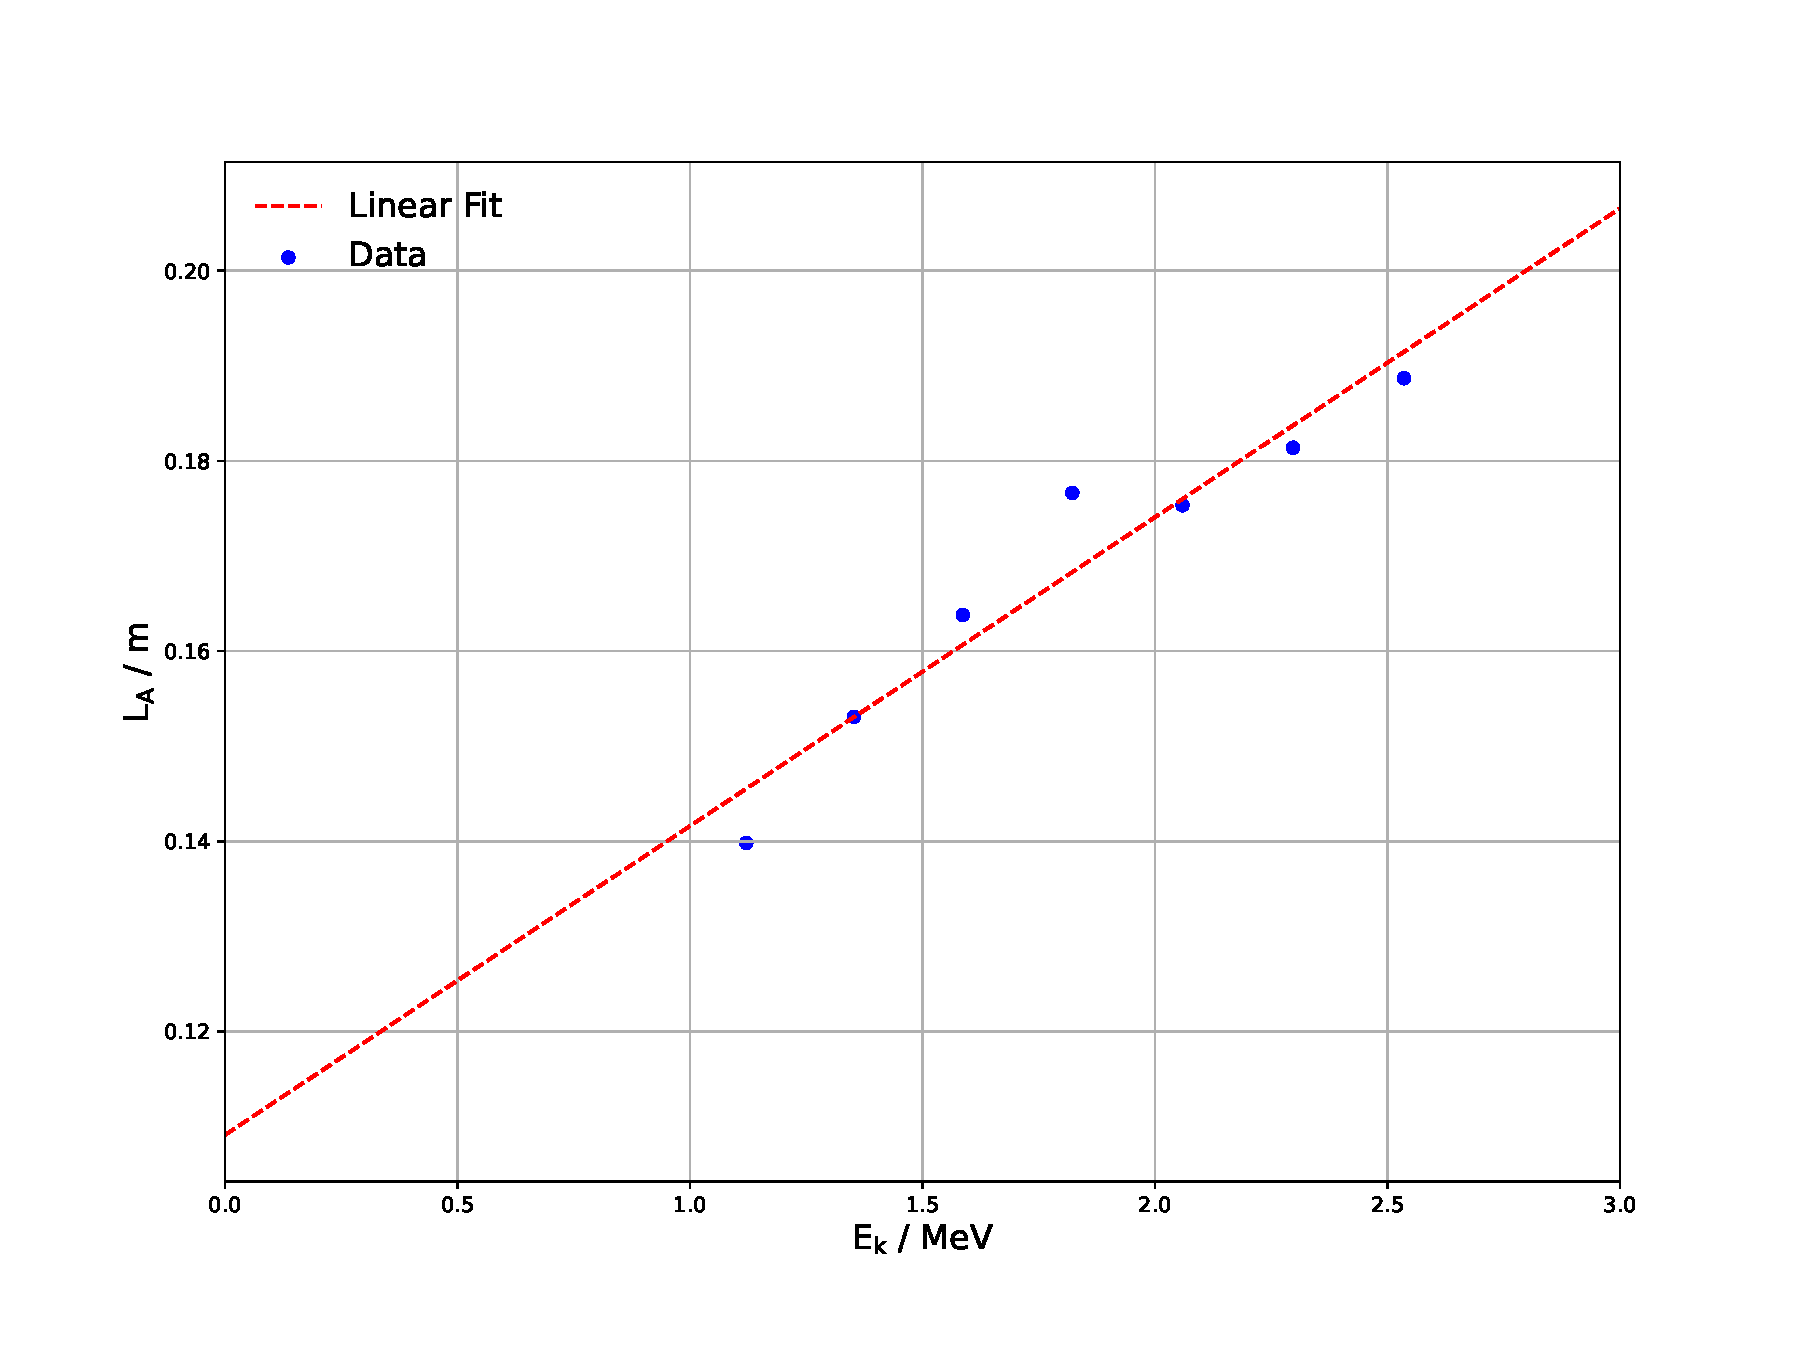
\includegraphics[height=12cm, width=16cm]{images/phyex6_fig3.pdf}
 \caption{空气对不同动能的$\beta$射线的衰减长度}
 \label{fig:fig12}
\end{figure}\\\\
可以看出能量越大, $\beta$射线的穿透能力越强, 即衰减长度的数值越大
%add more subsections for other block

%%%%%%%%%%%%%%%%%%%%%%%%%%%%%%%%%%%%%%%% Conclusion %%%%%%%%%%%%%%%%%%%%%%%%%%%%%%%%%%%%%%%%
\newpage
\section{结论}\label{conclusions}
由以上结果可见,$\beta$粒子在空气中的衰减长度$L_0$大致为三十几厘米,且$L_0$似乎随着粒子能动量(对应出射窗口编号)的增大而增大.

但可以确定的是,该能量范围的$\beta$粒子在 \SI{1}{atm} 下的衰减长度大致均在$30\sim40cm$上下,与$L$在同一量级, 这也进一步肯定了在真空环境中进行实验的必要性.

同时, 蒙卡模拟和实验数据测量得到的结果在一定程度上符合得比较好.

%%%%%%%%%%%%%%%%%%%%%%%%%%%%%%%%%%%%%%%% Questions %%%%%%%%%%%%%%%%%%%%%%%%%%%%%%%%%%%%%%%%
\begin{comment}
\section{实验报告思考题}\label{questions}
\subsection{在$a=23.0mm$、$b=10.0mm$的矩形波导管中能不能传播$\lambda=2cm$、$3cm$和$5cm$的微波?各能传播哪些波型?}\label{sub:question1}
答:根据
\begin{equation}
    \lambda_c=\frac{2}{\sqrt{(m/a)^2+(n/b)^2}}
\end{equation}
我们可以算出可传播的最大波长为$\lambda_{max}=18.3mm$,显然不能传播$\lambda=2cm$、$3cm$和$5cm$的微波,可传输波长在$\lambda_{max}=18.3mm$以下,满足$\lambda_c=\frac{2}{\sqrt{(m/a)^2+(n/b)^2}}$的波长的波型\\

\end{comment}

%%%%%%%%%%%%%%%%%%%%%%%%%%%%%%%%%%%%%%%% Acknowledgements %%%%%%%%%%%%%%%%%%%%%%%%%%%%%%%%%%%%%%%%

\section{致谢}\label{acknowledgments}
感谢王老师在实验中的的悉心指导.

\begin{comment}
%%%%%%%%%%%%%%%%%%%%%%%%%%%%%%%%%%%%%%%% Appendix %%%%%%%%%%%%%%%%%%%%%%%%%%%%%%%%%%%%%%%%
\appendix
\section{代码}\label{sub:app.code}
请在附录\ref{sub:app.code}中添加代码。请使用如下Scala的语法高亮描述方法。
\begin{scala}
class TopIO extends Bundle() {
	val boot = Input(Bool()) 
// imem and dmem interface for Tests
	val test_im_wr		= Input(Bool())
	val test_im_rd 		= Input(Bool())
	val test_im_addr 	= Input(UInt(32.W))
	val test_im_in 		= Input(UInt(32.W))
	val test_im_out 	= Output(UInt(32.W))

	val test_dm_wr		= Input(Bool())
	val test_dm_rd 		= Input(Bool())
	val test_dm_addr 	= Input(UInt(32.W))
	val test_dm_in 		= Input(UInt(32.W))
	val test_dm_out 	= Output(UInt(32.W))

	val valid			= Output(Bool())
}
class Top extends Module() {
	val io 		= IO(new TopIO())//in chisel3, io must be wrapped in IO(...) 
	//...
	when (io.boot & io.test_im_wr){
		imm(io.test_im_addr) := io.test_im_in
		} .elsewhen (io.boot & io.test_dm_wr){
		// please finish it
		} //...
}
\end{scala}
\newpage

%%%%%%%%%%%%%%%%%%%%%%%%%%%%%%%%%%%%%%%% REFERENCE %%%%%%%%%%%%%%%%%%%%%%%%%%%%%%%%%%%%%%%%
\begin{thebibliography}{9}

\bibitem{Erdos01} P. Erd\H os, \emph{A selection of problems and
results in combinatorics}, Recent trends in combinatorics (Matrahaza,
1995), Cambridge Univ. Press, Cambridge, 2001, pp. 1--6.

\end{thebibliography}
\end{comment}
\end{document}

